        %%******************************************%%
        %%                                          %%
        %%        Modello di tesi di laurea         %%
        %%            di Andrea Giraldin            %%
        %%                                          %%
        %%             2 novembre 2012              %%
        %%                                          %%
        %%******************************************%%

\begin{document}
    \frontmatter
    \begin{titlepage}
    \begin{center}
        \begin{LARGE}
            \textbf{\myUni}\\
        \end{LARGE}

        \vspace{10pt}

        \begin{Large}
            \textsc{\myDepartment}\\
        \end{Large}

        \vspace{10pt}

        \begin{large}
            \textsc{\myFaculty}\\
        \end{large}

        \vspace{30pt}
        \begin{figure}[htbp]
            \centering
            
\includegraphics[height=6cm]{unipd-logo}
        \end{figure}
        \vspace{30pt}

        \begin{LARGE}
            \textbf{\myTitle}\\
        \end{LARGE}

        \vspace{10pt}

        \begin{large}
            \textsl{\myDegree}\\
        \end{large}

        \vspace{40pt}

        \begin{large}
            \begin{flushleft}
                \textit{Relatore}\\
                \vspace{5pt}
                \profTitle\ \myProf
                \vspace{10pt}\\
                \textit{Correlatore}\\
                \vspace{5pt}
                \tutorTitle\ \myTutor
            \end{flushleft}

            % You can tweak the spacing to have professor and student names on the same line
            % useful if the page is broken by a long thesis title and you need more space
            \vspace{-70pt}

            \begin{flushright}
                \textit{Laureando}\\
                \vspace{5pt}
                \myName \\
                \vspace{5pt}
                \textit{Matricola} \myID
            \end{flushright}
        \end{large}

        \vspace{30pt}

        \line(1, 0){338} \\
        \begin{normalsize}
            \textsc{Anno Accademico \myAA}
        \end{normalsize}
    \end{center}
\end{titlepage}

    \clearpage
\phantomsection
\thispagestyle{empty}

\hfill
\vfill

\noindent\myName: \textit{\myTitle,}
\myDegree,
\textcopyright\ \myTime.

    \cleardoublepage
\phantomsection
\thispagestyle{empty}
\pdfbookmark{Dedica}{Dedica}

\vspace*{3cm}

\begin{center}
         Dentro un ring o fuori, non c'è niente di male a cadere. È sbagliato rimanere a terra. \\ \medskip
    --- Muhammad Ali
\end{center}

\medskip

\begin{center}
    Dedicato a Luigino
\end{center}

    \cleardoublepage
\phantomsection
\pdfbookmark{Sommario}{Sommario}
\begingroup
\let\clearpage\relax
\let\cleardoublepage\relax
\let\cleardoublepage\relax

\chapter*{Sommario}

Il presente documento si propone di descrivere il lavoro svolto durante il periodo di stage, della durata di circa trecento ore, dal laureando Alessandro Passarella presso l'azienda Salvagnini S.p.A. Lo scopo dello stage era quello di progettare e implementare un algoritmo genetico per ottimizzare il processo di nesting di forme regolari su lamiere metalliche. Il nesting è una tecnica utilizzata per disporre in modo efficiente elementi geometrici su superfici limitate, riducendo al minimo gli scarti di materiale. 

Il lavoro si articola in diverse fasi: inizialmente viene condotto uno studio della letteratura sugli algoritmi genetici, noti per la loro efficacia nella risoluzione di problemi di ottimizzazione combinatoria. Successivamente, si analizza il problema specifico di nesting affrontato dall'azienda e il codice esistente utilizzato per la sua risoluzione. Si procede quindi alla progettazione e implementazione di un algoritmo genetico che si integri con il software di ottimizzazione aziendale. Infine, i risultati ottenuti dall'algoritmo vengono confrontati con quelli di altre tecniche utilizzate dall'azienda attraverso un'analisi statistica, valutandone l'efficacia in termini di qualità delle soluzioni e tempi di esecuzione.

Questo lavoro offre un contributo significativo all'ottimizzazione dei processi di produzione nel settore della lavorazione delle lamiere, migliorando l'efficienza e riducendo gli sprechi di materiale.

%\vfill

%\selectlanguage{english}
%\pdfbookmark{Abstract}{Abstract}
%\chapter*{Abstract}

%\selectlanguage{italian}

\endgroup

\vfill

    \cleardoublepage
\phantomsection
\pdfbookmark{Ringraziamenti}{ringraziamenti}

\begingroup
\let\clearpage\relax
\let\cleardoublepage\relax
\let\cleardoublepage\relax

\chapter*{Ringraziamenti}

\noindent \textit{Innanzitutto, vorrei esprimere la mia gratitudine al Prof. \myProf, relatore della mia tesi, il gentilissimo dottor \myTutor, correlatore, e la dottoressa Chiara Turbian per l'aiuto e il sostegno fornitomi durante la stesura del lavoro.}\\

\noindent \textit{Desidero ringraziare la mia famiglia per il sostegno per il grande aiuto in ogni momento durante gli anni di studio.}\\

\bigskip

\noindent\textit{\myLocation, \myTime}
\hfill \myName

\endgroup

    \cleardoublepage
\pdfbookmark{\contentsname}{tableofcontents}
\setcounter{tocdepth}{2}
\tableofcontents
%\markboth{\contentsname}{\contentsname}
\clearpage

\begingroup
    \let\clearpage\relax
    \let\cleardoublepage\relax
    \let\cleardoublepage\relax

    % Figures list
    \phantomsection
    \pdfbookmark{\listfigurename}{lof}
    \listoffigures

    \vspace*{8ex}

    % Tables list
    \phantomsection
    \pdfbookmark{\listtablename}{lot}
    \listoftables

    \vspace*{8ex}
\endgroup

\cleardoublepage

    \cleardoublepage

    \mainmatter
    \chapter{Introduzione}
\label{cap:introduzione}

\intro{In questo capitolo verrà descritto brevemente il contesto in cui si è svolto lo stage, e come questo si è inserito nell’ottica aziendale.} \\

% \noindent Esempio di utilizzo di un termine nel glossario \\
% \gls{api}. \\

% \noindent Esempio di citazione in linea \\
% \cite{site:agile-manifesto}. \\

% \noindent Esempio di citazione nel pie' di pagina \\
% citazione\footcite{womak:lean-thinking} \\

\section{L'azienda} \hypertarget{salvagnini}{}

Il lavoro svolto in questa tesi fa riferimento al periodo di stage svolto presso Salvagnini Italia S.p.A. (da ora in poi abbreviata in Salvagnini). L'azienda, situata nel nord Italia, progetta, produce e commercializza Flexible Manufacturing System (FMS) costituiti da macchine a Controllo Numerico Computerizzato (CNC) per il taglio e la piegatura della lamiera, insieme a software dedicati. I processi in un FMS Salvagnini sono progettati per garantire una produzione personalizzata, massimizzando la produttività e minimizzando sprechi di materiali e consumi. In questo contesto, sorgono numerosi problemi di ottimizzazione, gestiti dal dipartimento di Ricerca e Sviluppo (R\&S)  [\hyperlink{bibliografia}{6}].

Da un lato, le macchine sono dotate di un numero crescente di processi automatizzati che eliminano i tempi morti e riducono le possibilità di errore. Dall'altro, una gran parte dell'ottimizzazione viene affrontata a livello software, attraverso lo sviluppo di applicazioni CAD (Computer-Aided Design) e CAM (Computer-Aided Manufacturing). Queste applicazioni assistono gli operatori con strumenti automatici per affrontare problemi complessi, come il modo in cui una macchina deve lavorare le lamiere, l'ordine in cui devono essere eseguite le operazioni, e così via.

\section{Scopo e contenuti dello stage}

L’attività di stage prevede lo studio, sviluppo e test di un algoritmo di ottimizzazione per la risoluzione di problemi di nesting di interesse nell’ambiente Salvagnini. In particolare, lo stage vuole verificare l'efficacia di un approccio basato su algoritmi genetici.
Occorre affrontare inizialmente lo studio della letteratura di Ricerca Operativa nell’ambito degli algoritmi genetici, un metodo evolutivo che classicamente ha riportato risultati significativi in problemi affini a quelli di interesse. Si passa poi alla definizione del problema di nesting in Salvagnini e all’analisi del codice sviluppato internamente per la risoluzione dello stesso. Avviene poi lo sviluppo di una versione dell’algoritmo genetico che risolva il problema di nesting in esame e che allo stesso tempo si integri nell’attuale software di ottimizzazione. Infine, verrà eseguita un’analisi statistica dei risultati prodotti da tale algoritmo, confrontandolo con altri metodi risolutivi già sviluppati dall’azienda, in termini di tempo di esecuzione e di qualità delle soluzioni proposte.

\section{Il problema del cutting stock nel contesto aziendale}

In Ricerca Operativa, il \emph{Cutting Stock Problem} (CSP) rappresenta una classe di \emph{problemi di ottimizzazione combinatoria}\glsfirstoccur di rilevanza pratica che coinvolge il posizionamento di oggetti più piccoli a oggetti più grandi, generalmente con l'obiettivo di minimizzare gli scarti. I problemi di CSP possono differire tra loro per una grande varietà di caratteristiche. Ad esempio, le dimensioni sia degli oggetti piccoli che di quelli grandi possono variare da 1 a 3 dimensioni. Il caso bidimensionale riguarda il taglio di oggetti (o parti) da fogli di materiale riducendo gli scarti, come avviene nelle industrie del legno, del vetro e della lamiera.

\subsection{Contesto}

Salvagnini produce essenzialmente due tipi di macchine da taglio, equipaggiate con tecnologie di taglio differenti: punzonatura e taglio laser. La tecnologia di punzonatura utilizza una macchina dotata di una testa multipressa che ospita diversi utensili rotanti per perforare la lamiera applicando alta pressione. Inoltre, le macchine di punzonatura Salvagnini presentano una cesoia di scarico integrata composta da due lame, indipendenti e ortogonali tra loro. La cesoia è in grado di tagliare qualsiasi lunghezza ed è utilizzata per staccare ogni pezzo lavorato dalla lamiera. Questa tecnologia di taglio è altamente efficiente per produrre diversi tipi di pezzi, tendenzialmente di forma regolare con eventuali scantonarure negli angoli. D'altra parte, le macchine da taglio laser hanno una testa ottica singola integrata con un sistema di raffreddamento a secco per controllare la temperatura delle ottiche, garantendo tagli estremamente precisi. La precisione del taglio laser consente di produrre forme intricate con dettagli fini e alta accuratezza [\hyperlink{bibliografia}{1}].

%[preso da chiara]

\subsection{Nesting}

Il Nesting è una forma particolare del CSP a due dimensioni, in cui delgli oggetti di piccola dimensione, di forma regolare o irregolare, possono essere liberamente posizionati su uno o piu oggetti di grandi dimensioni. In questa tesi ci concentriamo su forme regolari dato che nel caso Salvagnini facciamo riferimento alle macchine con taglio a punzonatura descritte in precedenza. 

Nel contesto dell’ottimizzazione del Nesting, occorre considerare una serie di vincoli che condizionano la disposizione degli elementi su un foglio. Alcuni di questi vincoli sono standard per questa tipologia di problema, mentre altri risultano specifici del caso Salvagnini. 

Naturalmente gli oggetti che vengono posizionati su uno stesso foglio non devono occupare aree comuni, garantendo così che ciascun elemento abbia il proprio spazio assegnato senza interferenze. Inoltre, ogni elemento deve mantenere una distanza minima dai bordi definiti del foglio, così come tra gli altri elementi, assicurando che vi sia sufficiente spazio per le operazioni di punzonatura senza compromettere la qualità del taglio o della lavorazione. Si aggiungono poi i \emph{margini di sicurezza}\glsfirstoccur, o \emph{margini per il taglio comune}\glsfirstoccur, che si applicano quando due elementi adiacenti non condividono un bordo. In tali situazioni, è essenziale rispettare una distanza di sicurezza che garantisca la corretta separazione dei pezzi durante la lavorazione, evitando sovrapposizioni o interferenze tra le traiettorie di taglio.

Dal punto di vista delle assegnazioni, vi sono due categorie di elementi: quelli obbligatori e quelli opzionali. Gli elementi obbligatori devono necessariamente essere collocati sul foglio, senza eccezioni. Gli elementi opzionali, invece, vengono utilizzati in funzione della riduzione degli \emph{scarti}\glsfirstoccur. Pertanto, questi ultimi possono non essere posizionati o possono essere posizionati solo alcuni, a seconda delle esigenze specifiche.

Un ulteriore vincolo importante riguarda le \emph{precedenze}\glsfirstoccur. In particolare, si distinguono due tipi di precedenza: hard e soft. A questo proposito, osserviamo che la soluzione potrebbe essere in generale composta da più fogli di lamiera, e che tra questi fogli è definito un ordine di produzione. I vincoli di precedenza richiedono che alcuni oggetti debbano essere posizionati in fogli che saranno prodotti prima di altri. Le precedenze hard stabiliscono che gli elementi con una priorità più alta devono essere posizionati seguendo l'ordine prestabilito. Questo ordine è rigido e non può essere infranto. Al contrario, le precedenze soft permettono una maggiore flessibilità: esse vanno rispettate solo qualora non comportino un aumento degli scarti. In caso contrario, possono essere infrante per ottimizzare l’utilizzo del materiale.

Infine, è necessario considerare le rotazioni consentite. Ogni elemento può essere ruotato per adattarsi meglio al layout, ma solo entro gli angoli permessi dagli strumenti di punzonatura (0°, 90°, 180° e 270°). Questo vincolo garantisce che le operazioni di lavorazione possano essere eseguite senza problemi e rispettando le specifiche tecniche degli strumenti.

Questi vincoli, considerati nel loro insieme, rappresentano un complesso sistema di regole che deve essere gestito attentamente per ottimizzare l’utilizzo del materiale e minimizzare gli scarti, garantendo al contempo che le specifiche di lavorazione vengano rispettate.

\section{Definizione del problema} \hypertarget{statement}{}

Di seguito è descritto il problema di nesting di forme regolari con tecnologia di taglio a punzonatura [\hyperlink{bibliografia}{9}], che è oggetto dello stage.

\begin{itemize}
    \item \textbf{Input}
    \begin{itemize}
        \item Dati sui fogli: larghezza, altezza, spessore, margini di sicurezza e quantità disponibile per ciascun tipo di foglio.
        \item Dati sugli elementi obbligatori: larghezza, altezza rotazioni consentite, zone di posizionamento proibite e obbligatorie, margini di punzonatura, livelli di precedenza hard e soft.
        \item Dati sugli elementi opzionali: larghezza, altezza, rotazioni consentite, zone di posizionamento proibite e obbligatorie, margini di punzonatura.
    \end{itemize}
    \item \textbf{Output}: sequenza di di layout di taglio.
    \item \textbf{Vincoli rigidi}
    \begin{itemize}
        \item Quantità massima dei tipi di foglio;
        \item Non sovrapposizione;
        \item Margini di punzonatura;
        \item Margini di sicurezza o taglio comune;
        \item Assegnazione degli elementi obbligatori;
        \item Assegnazione degli elementi opzionali;
        \item Precedenze hard;
        \item Rotazioni consentite;
        \item Vincoli su zone obbligatorie;
        \item Vincoli su zone proibite.
    \end{itemize}
    \item \textbf{Vincoli flessibili}: una soluzione ammissibile dovrebbe, a parità di scarto generato, rispettare il vincolo di precedenza soft.
    \item \textbf{Funzione obiettivo}: minimizzare la quantità totale di materiale scartato.
\end{itemize}


\section{Organizzazione del testo}

\begin{description}
    \item[{\hyperref[cap:processi-metodologie]{Il secondo capitolo}}] descrive i vincoli temporali e tecnologici, gli obiettivi, la pianificazione del lavoro e l'analisi dei rischi.
    
    \item[{\hyperref[cap:descrizione-stage]{Il terzo capitolo}}] tratta l'analisi della letteratura visionata per ottenere la soluzione al problema affrontato.
    
    \item[{\hyperref[cap:analisi-requisiti]{Il quarto capitolo}}] spiega le soluzioni di progettazione e la calibrazione dell'algoritmo.
    
    \item[{\hyperref[cap:progettazione-codifica]{Il quinto capitolo}}] mostra com'è stato implementato l'algoritmo.
    
    \item[{\hyperref[cap:verifica-validazione]{Il sesto capitolo}}] espone i test eseguiti e i risultati ottenuti.
    
    \item[{\hyperref[cap:conclusioni]{Nel settimo capitolo}}] viene valutata complessivamente l'esperienza, i risultati ottenuti, obiettivi raggiunti e conoscenze aquisite.
\end{description}

Riguardo la stesura del testo, relativamente al documento sono state adottate le seguenti convenzioni tipografiche:
\begin{itemize}
	\item gli acronimi, le abbreviazioni e i termini ambigui o di uso non comune menzionati vengono definiti nel glossario, situato alla fine del presente documento;
	\item per la prima occorrenza dei termini riportati nel glossario viene utilizzata la seguente nomenclatura: \emph{parola}\glsfirstoccur;
	\item i termini in lingua straniera o facenti parti del gergo tecnico sono evidenziati con il carattere \emph{corsivo}.
\end{itemize}

    \chapter{Processi e metodologie}
\label{cap:processi-metodologie}

\intro{In questo capitolo verranno riportati in modo approfondito lo scopo e gli obiettivi dello stage, contestualizzazione delle attività alla realtà aziendale e scadenzario delle stesse.}\\

\section{Definizione del problema}

In Ricerca Operativa, il \emph{Cutting Stock Problem} (CSP) rappresenta una classe di \emph{problemi di ottimizzazione combinatoria}\glsfirstoccur di rilevanza pratica che coinvolge l'assegnazione di oggetti più piccoli a oggetti più grandi, generalmente con l'obiettivo di minimizzare gli scarti. I problemi di CSP possono differire tra loro per una grande varietà di caratteristiche. Ad esempio, le dimensioni sia degli oggetti piccoli che di quelli grandi possono variare da 1 a 3 dimensioni. Il caso bidimensionale riguarda il taglio di oggetti (o parti) da fogli di materiale riducendo gli scarti, come avviene nelle industrie del legno, del vetro e della lamiera.

\subsection{Contesto}

Salvagnini produce essenzialmente due tipi di macchine da taglio, equipaggiate con tecnologie di taglio differenti: punzonatura e taglio laser. La tecnologia di punzonatura utilizza una macchina dotata di una testa multipressa che ospita diversi utensili rotanti per perforare la lamiera applicando alta pressione. Inoltre, le macchine di punzonatura Salvagnini presentano una cesoia di scarico integrata composta da due lame, indipendenti e ortogonali tra loro. La cesoia è in grado di tagliare qualsiasi lunghezza ed è utilizzata per staccare ogni pezzo lavorato dalla lamiera. Questa tecnologia di taglio è altamente efficiente per produrre diversi tipi di pezzi, tendenzialmente di forma regolare con eventuali scantonarure negli angoli. D'altra parte, le macchine da taglio laser hanno una testa ottica singola integrata con un sistema di raffreddamento a secco per controllare la temperatura delle ottiche, garantendo tagli estremamente precisi. La precisione del taglio laser consente di produrre forme intricate con dettagli fini e alta accuratezza.

%[preso da chiara]

\subsection{Nesting}

Il Nesting è una forma particolare del CSP a due dimenzioni, solitamente riguarda le forme irregolari. In questa tesi ci concentriamo su forme regolari dato che nel caso Salvagnini facciamo riferimento alle macchine con taglio a punzonatura descritte in precedenza. 

Nel contesto dell’ottimizzazione del Nesting, occorre considerare una serie di vincoli che condizionano la disposizione degli elementi su un foglio. Alcuni di questi vincoli sono standard per questa tipologia di problema, mentre altri risultano specifici del caso Salvagnini. 

Naturalmente gli oggetti che vengono posizionati su uno stesso foglio non devono occupare aree comuni, garantendo così che ciascun elemento abbia il proprio spazio assegnato senza interferenze. Inoltre, ogni elemento deve mantenere una distanza minima dai bordi definiti del foglio, così come tra gli altri elementi, assicurando che vi sia sufficiente spazio per le operazioni di punzonatura senza compromettere la qualità del taglio o della lavorazione. Si aggiungono poi i \emph{margini di sicurezza}\glsfirstoccur, o \emph{margini per il taglio comune}\glsfirstoccur, che si applicano quando due elementi adiacenti non condividono un bordo. In tali situazioni, è essenziale rispettare una distanza di sicurezza che garantisca la corretta separazione dei pezzi durante la lavorazione, evitando sovrapposizioni o interferenze tra le traiettorie di taglio.

Dal punto di vista delle assegnazioni, vi sono due categorie di elementi: quelli obbligatori e quelli opzionali. Gli elementi obbligatori devono necessariamente essere collocati sul foglio, senza eccezioni. Gli elementi opzionali, invece, vengono utilizzati in funzione della riduzione degli \emph{scarti}\glsfirstoccur. Pertanto, questi ultimi possono non essere posizionati o possono essere posizionati solo alcuni, a seconda delle esigenze specifiche.

Un ulteriore vincolo importante riguarda le \emph{precedenze}\glsfirstoccur. In particolare, si distinguono due tipi di precedenza: hard e soft. Le precedenze hard stabiliscono che gli elementi con una priorità più alta devono essere posizionati prima di quelli con priorità più bassa. Questo ordine è rigido e non può essere infranto. Al contrario, le precedenze soft permettono una maggiore flessibilità: esse vanno rispettate solo qualora non comportino un aumento degli scarti. In caso contrario, possono essere infrante per ottimizzare l’utilizzo del materiale.

Infine, è necessario considerare le rotazioni consentite. Ogni elemento può essere ruotato per adattarsi meglio al layout, ma solo entro gli angoli permessi dagli strumenti di punzonatura (0°, 90°, 180° e 270°). Questo vincolo garantisce che le operazioni di lavorazione possano essere eseguite senza problemi e rispettando le specifiche tecniche degli strumenti.

Questi vincoli, considerati nel loro insieme, rappresentano un complesso sistema di regole che deve essere gestito attentamente per ottimizzare l’utilizzo del materiale e minimizzare gli scarti, garantendo al contempo che le specifiche di lavorazione vengano rispettate.

\section{Vincoli temporali e tecnologici}

L'unico vincolo tecnologico che mi è stato imposto è stato lo sviluppo dell'algoritmo tramite il linguaggio \emph{Python}\glsfirstoccur. Questo perché python rendere il processo di sviluppo più efficiente, infatti, è particolarmente adatto al \emph{fast prototyping}\glsfirstoccur, dato che non necessita di compilazione, a differenza di linguaggi come C++ e Java, e, inoltre, permette di avere maggiore flessibilità del codice grazie anche dall'uso dei \emph{notebook}\glsfirstoccur.

Prima di iniziare lo stage è stato concordato con l’azienda un piano di lavoro su un totale di 304 ore, lavorando 5 giorni a settimana, 8 ore per ciascun giorno eccetto il venerdì che per politica aziendale prevede 6,5 ore. 

\section{Obiettivi}

Ogni obiettivo è provvisto di un codice identificativo formato da una delle seguenti stringhe \textbf{OB}, \textbf{DE} e \textbf{FA}, che rappresentano il livello di importanza e da un numero incrementale positivo, che rispetta la seguente nomenclatura:
\begin{center}
    [Importanza][Identificativo]
\end{center}
Gli obbiettivi rappresentano ciò che vogliamo ottenere dell'attività di stage e sono divisi, a seconda dell'importanza, come segue:
\begin{itemize}
    \item Obiettivi obbligatori \textbf{(OB)}: 
    Rappresentano gli obiettivi vincolanti che dovranno essere necessariamente soddisfatti;
    \item Obiettivi desiderabili \textbf{(DE)}:
    Rappresentano gli obiettivi non vincolanti ma dal riconoscibile valore aggiunto;
    \item Obiettivi facoltativi \textbf{(FA)}:
    Rappresentano gli obiettivi facoltativi non vincolanti ma dal valore aggiunto non strettamente competitivo.
\end{itemize}
Ogni obbiettivo è affiancato da una breve descrizione.


\begin{table}[H]
\centering
\begin{tabular}{|l|p{10cm}|}
\hline
\textbf{Obiettivo} & \textbf{Descrizione} \\ \hline
OB1 & Studio e conoscenza di algoritmi euristici e metaeuristici nella letteratura della Ricerca Operativa \\ \hline
OB2 & Definizione del problema di nesting in esame \\ \hline
OB3 & Conoscenza del \emph{framework}\glsfirstoccur fornito dall’azienda con funzionalità di natura geometrica e di ottimizzazione nel contesto del nesting \\ \hline
OB4 & Implementazione di un algoritmo genetico per la risoluzione del problema di nesting in esame \\ \hline
OB5 & Verifica su \emph{benchmark}\glsfirstoccur aziendali dell’algoritmo, confrontandolo con soluzioni ottenute da altri metodi risolutivi interni all’azienda \\ \hline
OB6 & Documentazione del codice e manuale di utilizzo dei moduli sviluppati \\ \hline
\end{tabular}
\caption{Obiettivi Obbligatori}
\end{table}

\begin{table}[H]
\centering
\begin{tabular}{|l|p{10cm}|}
\hline
\textbf{Obiettivo} & \textbf{Descrizione} \\ \hline
DE1 & Analisi statistica per una validazione rigorosa e valutazione della significatività dei risultati ottenuti \\ \hline
\end{tabular}
\caption{Obiettivi Desiderabili}
\end{table}

\begin{table}[H]
\centering
\begin{tabular}{|l|p{10cm}|}
\hline
\textbf{Obiettivo} & \textbf{Descrizione} \\ \hline
FA1 & Adattamento e test dell'algoritmo genetico sviluppato su problemi di nesting simili a quello definito (ad esempio problemi con forme regolari/irregolari, strip packing) \\ \hline
\end{tabular}
\caption{Obiettivi Facoltativi}
\end{table}

\section{Pianificazione}

Divisione delle attività da svolgere con una stima in termini di ore della durata di ciascuna attività.\\

\begin{table}[H]
\centering
\begin{tabular}{|l|p{10cm}|}
\hline
\textbf{Durata in ore} & \textbf{Descrizione dell'attività} \\ \hline
30 & Studio della letteratura di Ricerca Operativa nell’ambito delle euristiche di ottimizzazione combinatoria e degli algoritmi genetici \\ \hline
10 & Studio delle tecnologie necessarie allo sviluppo dell’algoritmo di ottimizzazione (python, librerie di ottimizzazione) \\ \hline
60 & Definizione del problema di nesting e analisi degli algoritmi esistenti e della loro implementazione \\ \hline
130 & Sviluppo algoritmo genetico:
\begin{itemize}
    \item Progettazione degli operatori di codifica e decodifica delle soluzioni basati su euristiche costruttive (30 ore)
    \item Progettazione degli operatori di fitness, selezione e rimpiazzo generazionale (10 ore)
    \item Implementazione delle componenti algoritmiche (80 ore)
    \item Test degli algoritmi implementati su istanze di prova (10 ore)
\end{itemize} \\ \hline
44 & Test dell'algoritmo sviluppato su benchmark di letteratura e aziendali. Analisi statistica dei risultati prodotti su diversi benchmark confrontandoli con quelli dei metodi sviluppati dall'azienda \\ \hline
30 & Stesura documentazione codice e manuale di utilizzo dei modelli sviluppati \\ \hline
\textbf{Totale: 304 ore} & \\ \hline
\end{tabular}
\caption{Pianificazione del lavoro}
\end{table}

\section{Ambiente di lavoro}

Di seguito verranno esposti brevemente il ciclo di vita e la gestione del progetto, considerando anche l'ambiente di sviluppo.
\subsection{Metodo di sviluppo}
Il ciclo di vita dell'algoritmo he seguito i seguenti passi:
\begin{itemize}
    \item Comprensione del problema: definizione del problema di nesting;
    \item Analisi letteratura: lettura articoli accademici di algoritmi genetici;
    \item Sviluppo: implementazione dell'algoritmo;
    \item Verifica: testing massivo e verifica della soluzione fornita.
\end{itemize}

\subsection{Gestione di progetto}

In generale per la gestione della comunicazione, condivisione di informazioni, documentazione e articoli si è fatto uso dell’applicazione \emph{Microsoft Teams}\glsfirstoccur, per il versionamento e la gestione dei task si è fatto uso del servizio \emph{GitHub}\glsfirstoccur, infine per quanto riguarda l’interfaccia con cui versionare ho utilizzato \emph{GitHub Desktop}\glsfirstoccur.

\subsection{Linguaggio di programmazione e ambiente di sviluppo}

Per la fase iniziale dell'implementazione si è lavorato utilizzando \emph{Jupyter Notebook}\glsfirstoccur oppure, con il quale è stato possibile scrivere metodi in linguaggio Python in modo molto agevole. Quando l'algoritmo ha raggiunto una certa completezza è stato necessario raggruppare i vari metodi in più classi e iniziare a lavorare su VisualStudio Code all'algoritmo e su Jupyter Notebook ai test da effettuare.
Python è un linguaggio di programmazione orientato agli oggetti ed interpretato dinamicamente al momento dell’esecuzione da un interprete. Python risulta veramente versatile in quanto fornisce incredibili funzionalità utilizzabili in modo semplice e intuitivo, inoltre, dispone di moltissime librerie che permettono le più svariate operazioni, come: metodi per l'analisi statistica, la manipolazione dei dati, la creazione di grafici e operazioni sui file. 
Le principali librerie utilizzate sono: random (per l'utilizzo delle funzioni randomiche), pandas (per la manipolazione e analisi dei dati), matplotlib (per la visualizzazione dei risultati ottenuti nei test) e statsmodel (per l'analisi statistica).
\emph{VisualStudio Code}\glsfirstoccur è stato scelto per rendere agevole l'implementazione è stato utilizzato infatti, grazie alle sue estensioni, risulta molto versatile e completo. In particolare sono state usate estensioni generiche per python ma anche per l'uso dei notebook direttamente da VSCode e per la gestione dei file formato \emph{csv}\glsfirstoccur, usati nella fase di test.

\section{Analisi dei rischi}

Questa sezione del documento si concentra sull’analisi delle potenziali difficoltà che potrebbero emergere durante il corso dello stage, con l’obiettivo di identificare, analizzare e prevenire eventuali ostacoli o rallentamenti che potrebbero comprometterne il progresso complessivo. Per affrontare queste possibili problematiche, si è scelto di esaminare attentamente ciascun rischio, fornendo dettagli quali la descrizione del rischio, il grado di rischio associato, la pericolosità, le precauzioni da adottare e una possibile soluzione. Il grado di rischio definisce la possibilità di occorrenza dello stesso e varia da una scala crescente da 1 a 5, mentre la pericolosità varia tra “Alta”, “Media” e “Bassa”. 

Le informazioni vengono presentante in forma tabellare, in modo da facilitarne il monitoraggio continuo durante l’intero ciclo di vita del progetto. Ogni rischio è provvisto di un codice identificativo formato da una delle seguenti stringhe \textbf{RP}, \textbf{RO} e \textbf{RT}, che rappresentano la categoria di rischo e da un numero incrementale positivo. Le principali categorie di rischi considerate includono:
\begin{itemize}
    \item Rischi personali \textbf{(RP)};
    \item Rischi organizzativi \textbf{(RO)};
    \item Rischi tecnologici/software \textbf{(RT)}.
\end{itemize}
I rischi rispettano la seguente nomenclatura:
\begin{center}
    [Categoria][Identificativo]
\end{center}

\risk{RP1 - Mancanza di competenze tecniche specifiche}
{Mancanza di esperienze professionali nella realizzazione dell'algoritmo. Mancanza di conoscenze delle tecnologie necessarie allo sviluppo del prodotto.}
{2}
{Alta}
{Fase iniziale di studio delle tecnologie.}
{Comunicazione con tutor aziendale per concordare misure di adattamento.}

\risk{RP2 - Mancanza di conoscenze teoriche specifiche}
{Mancanza di conoscenze relative al problema in questione. Mancanza di conoscenza specifiche dell'ambito industriale.}
{5}
{Media}
{Fase iniziale di studio del problema di nesting e dell'approccio aziendale.}
{Comunicazione con tutor aziendale per concordare misure di adattamento.}

\risk{RP3 - Salute e malattia}
{Malattia o problematiche di salute mentale. Questa problematica potrebbe essere poco evidente dato lo svolgersi dello stage in periodo estivo ma particolarmente impattante dato il calendario fissato di giorni lavorativi.}
{1}
{Alta}
{-}
{Concordare con l'azienda giorni extra per raggiungere le ore previste.}

\risk{RO1 - Fornitura}
{Ritardi nella fornitura di risorse esterne. Mancato accesso a strumenti o risorse software necessari per lo sviluppo.}
{3}
{Alta}
{Comunicazioni rapide e chiare, misure di approvvigionamento alternative. Invio di domande e/o richieste di materiale all'azienza.}
{Comunicazione con tutor aziendale e azienza per concordare misure di adattamento.}

\risk{RO2 - Organizzazione attività inefficiente}
{Errori di valutazione in termini di tempistiche per lo svolgimento delle diverse attività pianificate.}
{2}
{Media}
{Studio a monte delle fasi di sviluppo e test dell'algoritmo.}
{Comunicazione con tutor aziendale per concordare misure di adattamento.}

\risk{RT1 - Incompatibilità tra diverse tecnologie o componenti software}
{Situazione presentante difficoltà nell’integrare le diverse tecnologie coinvolte.}
{1}
{Media}
{Studio a monte delle tecnologie e conseguente scelta ragionata delle stesse.}
{Comunicazione con tutor aziendale per concordare misure di adattamento.}

\risk{RT2 - Aggiornamenti o modifiche agli strumenti tecnologici in uso}
{Situazione nella quale alcune tecnologie individuate risultino indisponibili o aventi modifiche sostanziali potenzialmente invalidanti il lavoro svolto fino a quel punto.}
{1}
{Alta}
{Scelta ponderata delle tecnologie. Costruire un ambiente flessibile ai cambiamenti.}
{Comunicazione con tutor aziendale per concordare misure di adattamento.}

    \chapter{Descrizione dello stage}
\label{cap:descrizione-stage}


    \chapter{Modellazione del problema}
\label{cap:analisi-requisiti}

\intro{Questo capitolo espone una modellazione del problema da affrontare}

UNO! deve dire doveha preso il modello, CITANDO LA FOINTE

così la sua tesi è PLAGIO (se non cita le fonti, sta dicendo che ha fatto lei quello che scrive)

DUE
non credo che abbia senso un capitolo che riporta il modello, visto che poi non viene usatato. potrebbe riportare il modello in una sezione unica del capitolo 1, come supporto alla descerizione del problema

\section{Dichiarazione del problema}

Il problema descritto in seguito riguarda il nesting di forme regolari con tecnologia di taglio a punzonatura.

\begin{itemize}
    \item \textbf{Input}
    \begin{itemize}
        \item Dati sui fogli: larghezza, altezza, spessore, margini di sicurezza e quantità disponibile per ciascun tipo di foglio.
        \item Dati sugli elementi obbligatori: larghezza, altezza rotazioni consentite, zone di posizionamento proibite e obbligatorie, margini di punzonatura, livelli di precedenza hard e soft.
        \item Dati sugli elementi opzionali: larghezza, altezza, rotazioni consentite, zone di posizionamento proibite e obbligatorie, margini di punzonatura.
    \end{itemize}
    \item \textbf{Output}: sequenza di di layout di taglio.
    \item \textbf{Vinvoli rigidi}
    \begin{itemize}
        \item Quantità massima dei tipi di foglio;
        \item Non sovrapposizione;
        \item Margini di punzonatura;
        \item Margini di sicurezza o taglio comune;
        \item Assegnazione degli elementi obbligatori;
        \item Assegnazione degli elementi opzionali;
        \item Precedenze hard;
        \item Rotazioni consentite;
        \item Vincoli su zone obbligatorie;
        \item Vincoli su zone proibite.
    \end{itemize}
    \item \textbf{Vincoli flessibili}: una soluzione ammissibile dovrebbe, a parità di scarto generato, rispettare il vincolo di precedenza soft.
    \item \textbf{Funzione obiettivo}: minimizzare la quantità totale di materiale scartato.
\end{itemize}

\section{Modello}

\subsection*{1. Input}

\paragraph*{Dati sui fogli}  
\begin{itemize}
    \item \( T \): insieme dei tipi di fogli disponibili, dove ogni foglio \( t \in T \) è definito da:
    \begin{itemize}
        \item \( w_t \): larghezza del foglio \( t \),
        \item \( h_t \): altezza del foglio \( t \),
        \item \( s_t \): spessore del foglio \( t \),
        \item \( m_t \): margini di sicurezza del foglio \( t \),
        \item \( q_t \): quantità disponibile del foglio \( t \).
    \end{itemize}
\end{itemize}

\paragraph*{Dati sugli elementi obbligatori}  
\begin{itemize}
    \item \( E_O \): insieme degli elementi obbligatori, dove ogni elemento \( i \in E_O \) è definito da:
    \begin{itemize}
        \item \( w_i \): larghezza dell’elemento \( i \),
        \item \( h_i \): altezza dell’elemento \( i \),
        \item \( R_i \): insieme delle rotazioni consentite per l’elemento \( i \),
        \item \( Z_{p,i} \): insieme delle zone proibite per l’elemento \( i \),
        \item \( Z_{m,i} \): insieme delle zone obbligatorie per l’elemento \( i \),
        \item \( p_i \): margini di punzonatura dell’elemento \( i \),
        \item \( \text{priority}_i \): livello di precedenza hard o soft.
    \end{itemize}
\end{itemize}

\paragraph*{Dati sugli elementi opzionali}  
\begin{itemize}
    \item \( E_P \): insieme degli elementi opzionali, dove ogni elemento \( j \in E_P \) è definito da:
    \begin{itemize}
        \item \( w_j \): larghezza dell’elemento \( j \),
        \item \( h_j \): altezza dell’elemento \( j \),
        \item \( R_j \): insieme delle rotazioni consentite per l’elemento \( j \),
        \item \( Z_{p,j} \): insieme delle zone proibite per l’elemento \( j \),
        \item \( Z_{m,j} \): insieme delle zone obbligatorie per l’elemento \( j \),
        \item \( p_j \): margini di punzonatura dell’elemento \( j \).
    \end{itemize}
\end{itemize}

\subsection*{2. Variabili di Decisione}
\begin{itemize}
    \item \( x_{i,t} \): coordinata \( x \) dell’elemento \( i \) sul foglio \( t \),
    \item \( y_{i,t} \): coordinata \( y \) dell’elemento \( i \) sul foglio \( t \),
    \item \( r_{i,t} \in R_i \): rotazione applicata all’elemento \( i \) sul foglio \( t \),
    \item \( u_{i,t} \in \{0,1\} \): variabile binaria che vale 1 se l’elemento \( i \) è posizionato sul foglio \( t \), 0 altrimenti,
    \item \( s_t \): quantità di materiale scartato per il foglio \( t \).
\end{itemize}

\subsection*{3. Output}
La soluzione è definita come una sequenza di layout di taglio, che specifica:
\begin{itemize}
    \item Posizione (\( x_{i,t}, y_{i,t} \)),
    \item Rotazione \( r_{i,t} \),
    \item Tipo di foglio \( t \).
\end{itemize}

\subsection*{4. Vincoli Rigidi}

\paragraph*{1. Quantità massima dei tipi di foglio:}
\[
\sum_{t \in T} u_{i,t} \leq q_t, \quad \forall i \in E_O \cup E_P
\]

\paragraph*{2. Non sovrapposizione:}
Per ogni coppia di elementi \( i, j \) sullo stesso foglio \( t \):
\[
(x_{i,t} + w_i \leq x_{j,t}) \lor (x_{j,t} + w_j \leq x_{i,t}) \lor (y_{i,t} + h_i \leq y_{j,t}) \lor (y_{j,t} + h_j \leq y_{i,t})
\]

\paragraph*{3. Margini di punzonatura:}
\[
x_{i,t} \geq p_i, \quad y_{i,t} \geq p_i, \quad x_{i,t} + w_i \leq w_t - p_i, \quad y_{i,t} + h_i \leq h_t - p_i
\]

\paragraph*{4. Margini di sicurezza o taglio comune:}
Per ogni coppia di elementi \( i, j \) non adiacenti:
\[
\text{Distanza}(i,j) \geq m_t
\]

\paragraph*{5. Assegnazione degli elementi obbligatori:}
\[
\sum_{t \in T} u_{i,t} = 1, \quad \forall i \in E_O
\]

\paragraph*{6. Precedenze hard:}
\[
\text{priority}_i > \text{priority}_j \implies x_{i,t} + y_{i,t} < x_{j,t} + y_{j,t}, \quad \forall i,j \in E_O
\]

\paragraph*{7. Rotazioni consentite:}
\[
r_{i,t} \in R_i, \quad \forall i \in E_O \cup E_P
\]

\paragraph*{8. Zone proibite e obbligatorie:}
\[
(x_{i,t}, y_{i,t}) \in Z_{m,i}, \quad (x_{i,t}, y_{i,t}) \not\in Z_{p,i}
\]

\subsection*{5. Vincoli Flessibili}

\paragraph*{Precedenze soft:}
\[
\text{priority}_i > \text{priority}_j \implies x_{i,t} + y_{i,t} < x_{j,t} + y_{j,t}, \quad \text{se } s_t \text{ rimane costante.}
\]

\subsection*{6. Funzione Obiettivo}
Minimizzare la quantità totale di materiale scartato:
\[
\text{Minimizza } S = \sum_{t \in T} s_t
\]
dove:
\[
s_t = w_t \cdot h_t - \sum_{i \in E_O \cup E_P} (w_i \cdot h_i \cdot u_{i,t})
\]



% \intro{Breve introduzione al capitolo}\\

% \section{Casi d'uso}

% Per lo studio dei casi di utilizzo del prodotto sono stati creati dei diagrammi.
% I diagrammi dei casi d'uso (in inglese \emph{Use Case Diagram}) sono diagrammi di tipo \gls{uml} dedicati alla descrizione delle funzioni o servizi offerti da un sistema, così come sono percepiti e utilizzati dagli attori che interagiscono col sistema stesso.
% Essendo il progetto finalizzato alla creazione di un tool per l'automazione di un processo, le interazioni da parte dell'utilizzatore devono essere ovviamente ridotte allo stretto necessario. Per questo motivo i diagrammi d'uso risultano semplici e in numero ridotto.

% \begin{figure}[!h] 
%     \centering 
%     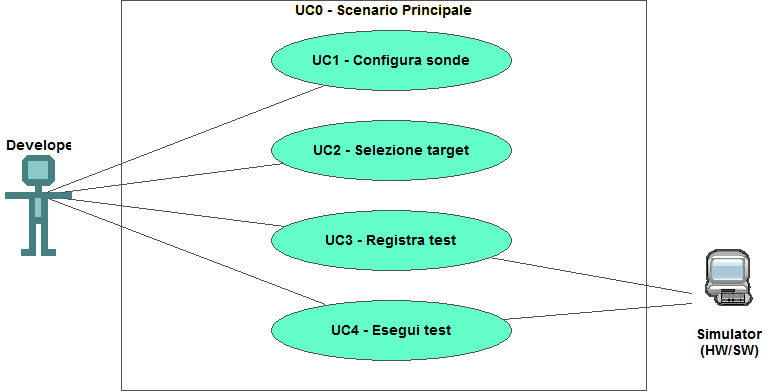
\includegraphics[width=0.9\columnwidth]{usecase/scenario-principale} 
%     \caption{Use Case - UC0: Scenario principale}
% \end{figure}

% \begin{usecase}{0}{Scenario principale}
% \usecaseactors{Sviluppatore applicativi}
% \usecasepre{Lo sviluppatore è entrato nel plug-in di simulazione all'interno dell'IDE}
% \usecasedesc{La finestra di simulazione mette a disposizione i comandi per configurare, registrare o eseguire un test}
% \usecasepost{Il sistema è pronto per permettere una nuova interazione}
% \label{uc:scenario-principale}
% \end{usecase}

% \section{Tracciamento dei requisiti}

% Da un'attenta analisi dei requisiti e degli use case effettuata sul progetto è stata stilata la tabella che traccia i requisiti in rapporto agli use case.\\
% Sono stati individuati diversi tipi di requisiti e si è quindi fatto utilizzo di un codice identificativo per distinguerli.\\
% Il codice dei requisiti è così strutturato R(F/Q/V)(N/D/O) dove:
% \begin{enumerate}
% 	\item[R =] requisito
%     \item[F =] funzionale
%     \item[Q =] qualitativo
%     \item[V =] di vincolo
%     \item[N =] obbligatorio (necessario)
%     \item[D =] desiderabile
%     \item[Z =] opzionale
% \end{enumerate}
% Nelle tabelle \ref{tab:requisiti-funzionali}, \ref{tab:requisiti-qualitativi} e \ref{tab:requisiti-vincolo} sono riassunti i requisiti e il loro tracciamento con gli use case delineati in fase di analisi.

% \newpage

% \begin{table}%
% \caption{Tabella del tracciamento dei requisti funzionali}
% \label{tab:requisiti-funzionali}
% \begin{tabularx}{\textwidth}{lXl}
% \hline\hline
% \textbf{Requisito} & \textbf{Descrizione} & \textbf{Use Case}\\
% \hline
% RFN-1     & L'interfaccia permette di configurare il tipo di sonde del test & UC1 \\
% \hline
% \end{tabularx}
% \end{table}%

% \begin{table}%
% \caption{Tabella del tracciamento dei requisiti qualitativi}
% \label{tab:requisiti-qualitativi}
% \begin{tabularx}{\textwidth}{lXl}
% \hline\hline
% \textbf{Requisito} & \textbf{Descrizione} & \textbf{Use Case}\\
% \hline
% RQD-1    & Le prestazioni del simulatore hardware deve garantire la giusta esecuzione dei test e non la generazione di falsi negativi & - \\
% \hline
% \end{tabularx}
% \end{table}%

% \begin{table}%
% \caption{Tabella del tracciamento dei requisiti di vincolo}
% \label{tab:requisiti-vincolo}
% \begin{tabularx}{\textwidth}{lXl}
% \hline\hline
% \textbf{Requisito} & \textbf{Descrizione} & \textbf{Use Case}\\
% \hline
% RVO-1    & La libreria per l'esecuzione dei test automatici deve essere riutilizzabile & - \\
% \hline
% \end{tabularx}
% \end{table}%

    \chapter{Progettazione e implementazione}
\label{cap:progettazione-codifica}

\lstset{
    escapeinside={(*@}{@*)}, % Delimitatori per modalità LaTeX
    basicstyle=\ttfamily,    % Stile monospaziato
}

\intro{Questo capitolo è incentrato sulla progettazione e sulla codifica dell'algoritmo, mostrando passo per passo il suo funzionamento}


\section{Progettazione}

Questa sezione esplora i diversi aspetti fondamentali nella progettazione di un algoritmo genetico: le componenti fondamentali, la struttura e gli operatori genetici.

\subsection{Composizione degli algoritmi evolutivi}

I principali componenti di ricerca per progettare un algoritmo evolutivo sono i seguenti:

\begin{itemize}
    \item \textbf{Rappresentazione}: negli algoritmi genetici, la soluzione codificata è chiamata cromosoma, mentre le variabili decisionali all'interno di una soluzione (cromosoma) sono i geni;
    
    \item \textbf{Inizializzazione della popolazione}: la generazione della popolazione iniziale è un aspetto cruciale in quanto una giusta inizializzazione determina un vantaggio già dalle prime interazioni;
    
    \item \textbf{Funzione di fitness}: si tratta della funzione obbiettivo, ogni soluzione ha un valore di fitness che indica il grado di adeguatezza rispetto al problema;
    
    \item \textbf{Strategia di selezione}: la strategia di selezione affronta la seguente domanda: "Quali genitori per la prossima generazione vengono scelti con un bias verso un fitness migliore?";
    
    \item \textbf{Strategia di riproduzione}: la strategia di riproduzione consiste nel progettare operatori di mutazione e crossover adeguati per generare nuovi individui (discendenti);
    
    \item \textbf{Strategia di sostituzione}: i nuovi discendenti competono con gli individui più vecchi per ottenere il loro posto nella prossima generazione (sopravvivenza del più adatto);
    
    \item \textbf{Criteri di arresto}: determina la fine del loop evolutivo, solitamente è indicato come il numero di generazioni da raggiungere, ovvero ogni interazione è una generazione.
\end{itemize}

\subsection{Struttura del genetico}

In questa sezione descriviamo la struttura dell'Algoritmo Genetico scelta per il controllo delle sue fasi di intensificazione e diversificazione.
L'obiettivo è massimizzare una funzione di fitness $f$. I parametri richiesti dall'algoritmo GA sono:

\begin{itemize}
    \item $N$: dimensione della popolazione;
    \item $p_c$: probabilità di crossover;
    \item $p_m$: probabilità di mutazione;
    \item $M$: dimensione del pool di accoppiamento;
    \item $E$: dimensione dell'élite.
\end{itemize}

Indichiamo con $P$ la popolazione di cromosomi e con $G$ l'insieme di discendenti generati dalla fase di riproduzione.

\begin{lstlisting}
def GA(N, pc, pm, M, E):
    P = generate(N);
    while not terminate() do
        G = reproduction(P, pc, pm, M);
        P = replace(P, G, E);
    end
    return maxf P;
end
\end{lstlisting}

\subsubsection{Riproduzione}
In questa fase utilizziamo operatori binari (crossover) e unari (mutazione) per esplorare altre soluzioni alterando solo una parte della soluzione. Questa modifica parziale (invece di una riorganizzazione totale, che sarebbe una ricerca casuale), insieme al sostegno degli individui più idonei (es. selezione dei genitori), porta l'algoritmo a spingere avanti nelle generazioni le soluzioni più idonee mantenendo un buon tasso di esplorazione di nuovi cromosomi. La dimensione dei discendenti richiesta è pari alla dimensione della popolazione $N$, che poi subisce la procedura di sostituzione.

La probabilità di riproduzione indicata con $Be(p)$, ovvero, la variabile casuale di Bernoulli che assume valore 1 con probabilità $p$ e 0 con probabilità $1-p$.

\begin{lstlisting}
    def Reproduction(P, pc, pm, M):
        G = [ ];
        pool = sortf(P)[0 : M];
        while not |G| == |P| do
            par1, par2 = selection(pool);
            if Be(pc) == 1 then
                c1, c2 = crossover(par1, par2);
            else
                c1, c2 = par1, par2;
            end
            G = G (*@$\cup$@*) {c1, c2};
        end
        foreach g (*@$\in$@*) G do
            if Be(pm) == 1 then
                mutation(c);
            end
        end
        return G;
    end
\end{lstlisting}

\subsubsection{Rimpiazzo}
La strategia di rimpiazzo ha un grande impatto sull'intensificazione. La metodologia di rimpiazzo adottata può essere spiegata in due passaggi: 
\begin{enumerate}
    \item i migliori $E$ elementi nell'unione di $P$ e $G$ fanno automaticamente parte della popolazione successiva;
    \item i migliori $|P| - E$ discendenti di $G$ sono inclusi nella popolazione successiva.
\end{enumerate}

\begin{lstlisting}
    def Replace(P, G, E):
        elite = best subset(P (*@$\cup$@*) G, E, f);
        Gbest = best subset(G, |P| - E, f);
        return elite (*@$\cup$@*) Gbest;
    end
\end{lstlisting}

\subsection{Operatori genetici}

Gli operatori genetici permettono agli algoritmi evolutivi di modulare la diversificazione. Operano sui cromosomi alterandone i geni e permettendo di esplorare un ampio spazio di soluzioni senza andare a perdere intensificazione grazie alla selezione e all'elitismo.

\subsubsection{Selezione}

La selezione dei genitori viene effettuata sui migliori \( M \) individui della popolazione attuale, i quali costituiscono il cosiddetto \emph{Mating Pool}.

Il meccanismo di selezione è uno dei principali componenti di ricerca negli algoritmi evolutivi (EAs). Il principio fondamentale dei metodi di selezione è: \emph{"più un individuo è valido, maggiore è la sua probabilità di essere scelto come genitore."} Questa pressione selettiva guida la popolazione verso soluzioni migliori. Tuttavia, gli individui peggiori non dovrebbero essere completamente scartati, poiché essi potrebbero contenere materiale genetico utile.

La strategia di selezione determina quali individui vengono scelti per l'accoppiamento (riproduzione).

La selezione tramite ruota della roulette è la strategia di selezione più comune. Essa assegna a ciascun individuo una probabilità di selezione proporzionale alla sua fitness relativa. Sia $f_i$ la fitness dell'individuo $p_i$ nella popolazione $P$. La probabilità di selezione è data da:

\[ p_i = \frac{f_i}{\sum_{j=1}^{n} f_j} \]

Immaginiamo un grafico a torta in cui a ciascun individuo è assegnato uno spazio proporzionale alla sua fitness. Una ruota della roulette è posizionata attorno al grafico. La selezione di $\mu$ individui avviene tramite $\mu$ spin indipendenti della ruota. Ogni spin seleziona un singolo individuo. Gli individui migliori occupano più spazio e, di conseguenza, hanno maggiori probabilità di essere scelti (Figura 5.2).

\begin{figure}[!ht] 
    \centering 
    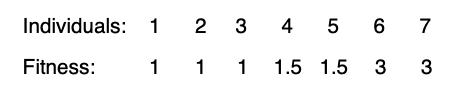
\includegraphics[width=0.6\columnwidth]{tesi/fitness_roulette_wheel} 
    \caption{Pesi della ruota}
\end{figure}

\begin{figure}[!ht] 
    \centering 
    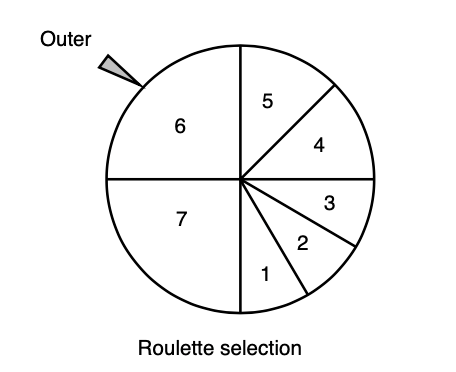
\includegraphics[width=0.6\columnwidth]{tesi/roulette_wheel} 
    \caption{Grafico a torta della selezione tramite ruota della roulette}
\end{figure}

Tuttavia, nella selezione tramite ruota della roulette, individui eccezionali possono introdurre un bias all'inizio della ricerca, causando una convergenza prematura e una perdita di diversità genetica. Infatti, va notato che un valore di \( M \) troppo piccolo intensifica il focus sui migliori individui del \emph{Mating Pool}, riducendo però la diversificazione della popolazione. Questo compromesso deve essere attentamente bilanciato per garantire un efficace equilibrio tra esplorazione e sfruttamento nel processo evolutivo.

\subsubsection{Crossover}
Il crossover prende i due genitori selezionati e genera due figli da aggiungere ai nuovi discendenti. Un crossover avviene con una probabilità $p_c$, altrimenti i genitori vengono semplicemente clonati e aggiunti ai discendenti. L'operatore di crossover, da un lato, mescola i geni delle coppie di cromosomi esplorando nuove soluzioni; dall'altro, se la diversità genetica (individui diversi) nella popolazione è bassa, può portare a una convergenza prematura. Nel caso estremo in cui abbiamo una popolazione composta da elementi tutti uguali, il crossover non può creare nuovi individui. Per garantire la diversità genetica, si può ridurre la fase di intensificazione (es. $E$ o $M$) o aumentare il tasso di mutazione $p_m$.

A differenza degli operatori unari, come la mutazione, l'operatore di crossover è binario e talvolta n-ario. Il ruolo degli operatori di crossover è di ereditare alcune caratteristiche dei due genitori per generare i discendenti. Come per l'operatore di mutazione, la progettazione degli operatori di crossover dipende principalmente dalla rappresentazione utilizzata.

Applicare operatori di crossover classici alle permutazioni, come nel nostro caso, genera soluzioni che non sono permutazioni (ossia, soluzioni non valide). Di conseguenza, sono stati progettati numerosi operatori di crossover per permutazioni, tra cui il crossover a ordine (OX). Per prima cosa, due punti di crossover vengono selezionati casualmente. Dal genitore 1, si copia nel discendente, alle stesse posizioni assolute, la parte tra i due punti. Dal genitore 2, si parte dal secondo punto di crossover e si scelgono gli elementi non già selezionati dal genitore 1, inserendoli nel discendente a partire dal secondo punto di crossover. L'operatore di crossover OX è un operatore di pura ricombinazione. Se si inizia a riempire o scegliere dal primo punto di crossover, l'operatore non sarà puro. Dal genitore 1, vengono preservati l'ordine relativo, l'adiacenza e le posizioni assolute. Dal genitore 2, viene preservato solo l'ordine relativo.

\begin{figure}[!ht] 
    \centering 
    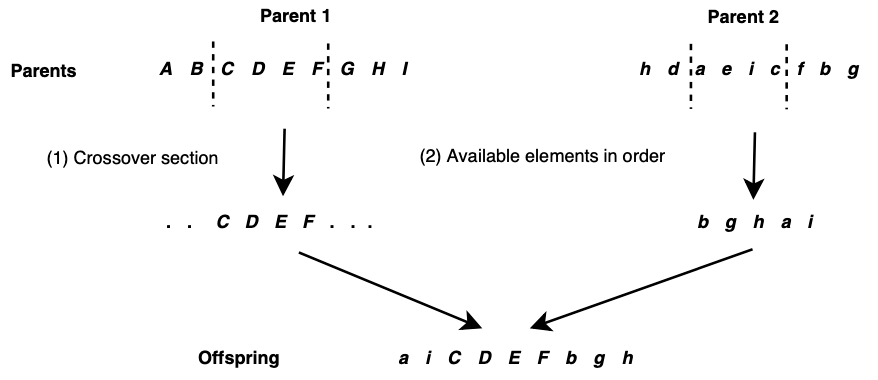
\includegraphics[width=1\columnwidth]{tesi/OXCrossover} 
    \caption{Rappresentazione del crossover OX}
\end{figure}

\subsubsection{Mutazione}
La mutazione viene eseguita dopo il crossover e crea una perturbazione casuale del cromosoma selezionato. Il ruolo della mutazione è duplice: da un lato, simile all'operatore di crossover, provoca una perturbazione di una soluzione per favorire l'esplorazione; dall'altro aumenta la diversità genetica anche se l'attuale diversità è scarsa. Questo è in contrasto con il crossover, che non può diversificare molto un set di individui molto simili.

Gli operatori di mutazione sono operatori unari che agiscono su un singolo individuo. Le mutazioni rappresentano piccoli cambiamenti degli individui selezionati nella popolazione. La probabilità $p_m$ definisce la probabilità di mutare ogni elemento (gene) della rappresentazione. Alcune strategie inizializzano la probabilità di mutazione a $1/k$, dove $k$ è il numero di variabili decisionali, in modo che in media solo poche variabili vengano mutate.

Alcuni punti importanti da considerare nella progettazione o nell'uso di un operatore di mutazione sono i seguenti:

\begin{itemize}
    \item \textbf{Ergodicità}: l'operatore di mutazione dovrebbe consentire di raggiungere ogni soluzione nello spazio di ricerca.
    \item \textbf{Validità}: l'operatore di mutazione dovrebbe produrre soluzioni valide. Questo non è sempre possibile nei problemi di ottimizzazione vincolati.
    \item \textbf{Località}: la mutazione dovrebbe produrre un cambiamento minimo. La dimensione della mutazione è importante e dovrebbe essere controllabile. La località è l'effetto sulla soluzione (fenotipo) quando si esegue la modifica (perturbazione) nella rappresentazione (genotipo). Quando vengono effettuati piccoli cambiamenti nel genotipo, il fenotipo deve rivelare piccoli cambiamenti. In questo caso, si dice che la mutazione ha una forte località. Una debole località è caratterizzata da un grande effetto sul fenotipo quando viene effettuato un piccolo cambiamento nel genotipo.
\end{itemize}

La mutazione in rappresentazioni basate sull'ordine, come nel nostro caso, è generalmente basata sugli operatori di scambio (swapping), inversione o inserimento. 

\section{Parametrizzazione}

In questa sezione viene discussa e motivata la scelta dei valori dei parametri dell'algoritmo tenendo contro delle caratteristiche da ottimizzare, delle istanze di prova fornite dall'azienda e di possibili rischi di overtuning.

L'obbiettivo è quello scegliere una configurazione ottimale di parametri dell'algoritmo per cercare di ottimizzare le seguenti caratteristiche:
\begin{itemize}
	\item\textbf{Intensificazione}: ci si aspetta che il valore di fitness della soluzione migliore all'interno della popolazione incrementi nel corso delle generazioni;
	\item\textbf{Diversificazione}: l'algoritmo deve esplorare un vasto insieme di soluzioni, gli operatori di crossover e mutazione potranno generare soluzioni con valori fitness inferiori a quello della peggiore soluzione della generazione precedente. Quando questo avviene significa che l'algoritmo sta esplorando anche soluzioni diverse, tuttavia non è necessariamente indice che l'esplorazione avvenga in maniera sufficente;
	\item\textbf{Costo computazionale}: come vedremmo in seguito, il criterio di arresto dei test svolti sull'algoritmo è un limite di tempo impostato a 30 secondi. In base all'istanza, è possibile che in 30 secondi vengano computizzate 10 o 100 generazioni. Siccome gli algoritmi genetici sono progettati per funzionare al meglio con l'incrementarsi di generazioni, il limite di tempo non è un criterio di arresto ottimale, tuttavia è necessario per confronti o test. Questo rende la velocità di esecuzione un aspetto di cui tenere conto per permettere all'algoritmo di eseguire più generazioni possibili nel tempo limite.
\end{itemize}

\subsection{Scelta delle configurazioni}

I parametri da configurare sono:
\begin{itemize}
	\item\textbf{population\_size}: dimensione della popolazione di cromosomi, ovvero le soluzioni sul quale lavora il genetico;
	\item\textbf{crossover\_prob}: probabilità che l'algoritmo svolga l'operazione di crossover (applicata a coppie di soluzioni presenti nella pool);
	\item\textbf{mutation\_prob}: probabilità che l'algoritmo svolga l'operazione di mutazione (applicata a ogni soluzione presente nella pool);
	\item\textbf{mating\_pool\_size}: dimensione del pool di accoppiamento;
	\item\textbf{elite\_size}: dimensione dell'insieme dei migliori cromosomi della popolazione che verranno inseriti direttamente nella popolazione della generazione successiva.
\end{itemize}

\noindent La configurazione iniziale (fornita dal tutor aziendale sulla base risultati ottenuti per un algoritmo genetico svolto su un altro problema) è, \textbf{Conf1}:
\begin{itemize}
	\item\textbf{population\_size}: 50;
	\item\textbf{crossover\_prob}: 0,7 (70\%);
	\item\textbf{mutation\_prob}: 0,3 (30\%);
	\item\textbf{mating\_pool\_size}: 20;
	\item\textbf{elite\_size}: 5.
\end{itemize}

Di seguito verranno mostrati alcuni grafici di test svolti su delle singole istanze di prova, fornite appositamente dall'azienda, allo scopo di mostrare l'andamento del valore di fitsess delle soluzioni della determinata istanza. Inoltre, per i test sui parametri dell'algoritmo è stato imposto un criterio di arresto non a limite di tempo ma a limite di generazioni, ed è stato fissato a 50 generazioni. 
L'asse y rappresenta il valore di fitness (da 0.75 a 0.95, dove 0 significa che lo spazio sprecato è tutto, e 1 che non c'è spazio sprecato). L'asse x rappresenta il numero di generazioni (da 0 a 50).
La trasparenza è regolata in modo che più sono presenti cromosomi maggiore è l'intensità del blu.

Dal seguente grafico (Figura 5.4) si nota come ci sia una buona diversificazione ma il valore di fitness della soluzione migliore converge troppo presto, infatti, intorno alla 15esima generazione stabilizza il valore di fitness della soluzione migliore. 

\begin{figure}[!ht] 
    \centering 
    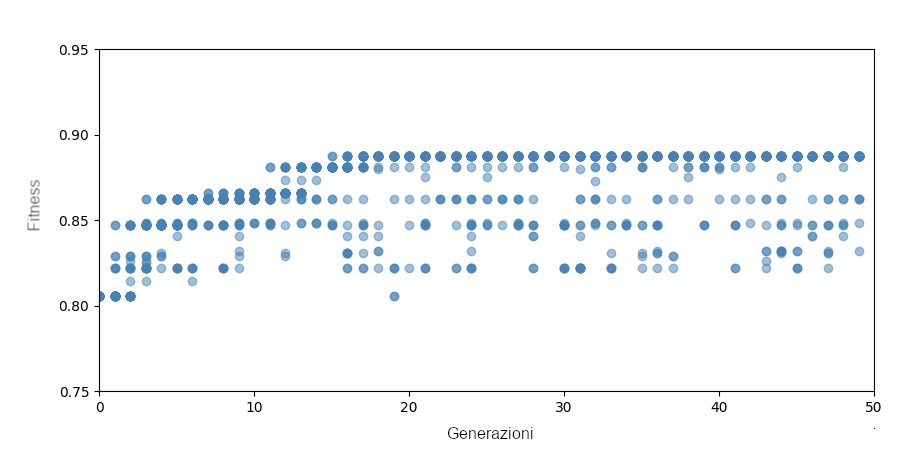
\includegraphics[width=1\columnwidth]{tesi/conf1} 
    \caption{Andamento valori di fitness di un instanza di prova testata con Conf1}
\end{figure}

\textbf{Conf2}:
\begin{itemize}
	\item\textbf{population\_size}: 50;
	\item\textbf{crossover\_prob}: 0,7 (70\%);
	\item\textbf{mutation\_prob}: 0,3 (30\%);
	\item\textbf{mating\_pool\_size}: 40;
	\item\textbf{elite\_size}: 5.
\end{itemize}

Per cercare subito un confronto la prima modifica è stata nella \emph{mating\_pool\_size}, portandola a 40 (da 20) (Figura 5.5), questo ha aumentato notevolmente la diversificazione ed ha trovato soluzioni con un valore di fitness migliore delle soluzioni migliori con la Conf1. 

\begin{figure}[!ht] 
    \centering 
    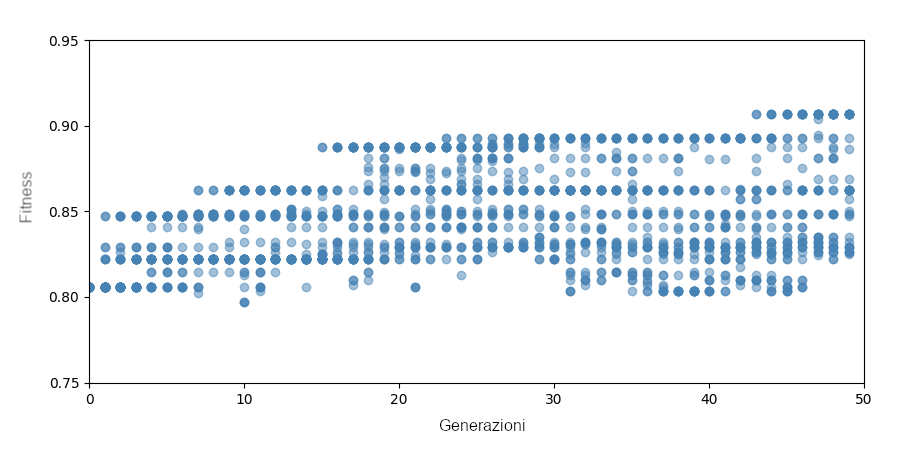
\includegraphics[width=1\columnwidth]{tesi/conf2} 
    \caption{Andamento valori di fitness di un instanza di prova testata con Conf2}
\end{figure}

Questo ha indicato come sicuramente sono presenti soluzioni migliori ottenibili con lo stesso numero di generazioni. Come si può notare, la Conf2 ha molta diversificazione, quindi l'obbiettivo di una nuova configurazione era migliorare l'intensificazione e cercare di diminuire la diversificazione senza perdere le nuove soluzioni che hanno ottenuto un valore di fitness migliore. Si è provato a diminuire la \emph{mating\_pool\_size} e aumentare la \emph{elite\_size} per aumentare l'intensificazione, ma è stato chiaro da subito che un 10\% di \emph{elite\_size} era già il massimo ottenibile senza ridurre drasticamente la diversificazione. Quindi si è provato ad aumentare \emph{crossover\_prob} ma con scarso successo. Sono state tentate anche configurazioni con diverse \emph{mutation\_prob} ma diminuendola si notava chiaramente un appiettimento della diversificazione, mentre, non si rendeva necessario aumentarla dato che un aumento della \emph{mating\_pool\_size} è sufficente per ottenere un giusto livello di diversificazione e aumenta anche l'intensificazione grazie al crossover.

\noindent L'equilibrio è stato trovato con la \textbf{Conf3}:
\begin{itemize}
	\item\textbf{population\_size}: 50;
	\item\textbf{crossover\_prob}: 0,7 (70\%);
	\item\textbf{mutation\_prob}: 0,3 (30\%);
	\item\textbf{mating\_pool\_size}: 30;
	\item\textbf{elite\_size}: 5.
\end{itemize}

(Figura 5.6), una \emph{mating\_pool\_size} corrispondente al 60\% della popolazione, ha generato un bilanciamento ottimale fra intensificazione, diversificazione e velocità di esecuzione. Infatti un altro problema della Conf2, era che una \emph{mating\_pool\_size} di 40 faceva svolgere una generazione in molto più tempo rispetto alla Conf1, quindi, essendo che i test di confronto con la soluzione aziendale, sarebbero stati svolti non con un criterio di arresto basato sulle generazione ma sul tempo, è stato necessario diminuire la \emph{mating\_pool\_size}.

\begin{figure}[!ht] 
    \centering 
    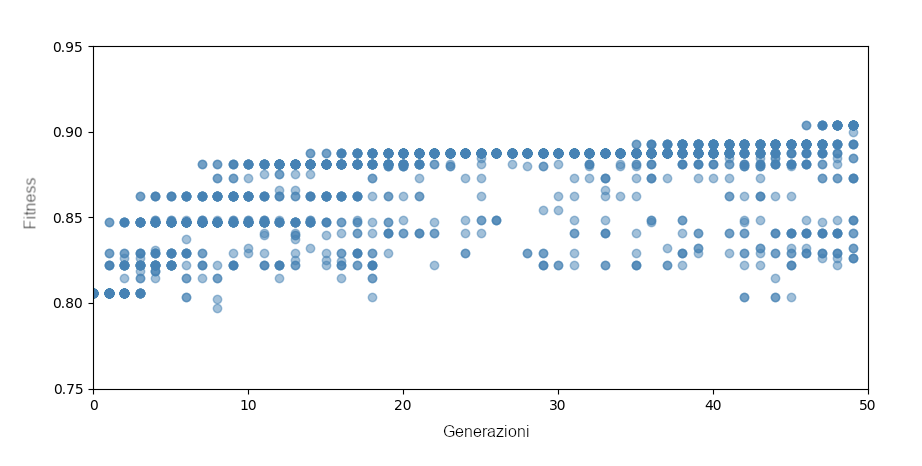
\includegraphics[width=1\columnwidth]{tesi/conf3} 
    \caption{Andamento valori di fitness di un instanza di prova testata con Conf3}
\end{figure}

\subsection{Analisi statistica}

50 istanze di prova diverse generate randomicamente, ciascusa istanza ha:
\begin{itemize}
	\item 1 solo tipo di foglio;
	\item 20 item obbligatori più 0 o 6 o 12 item opzionali;
	\item 0 o metà o tutti gli item obbligatori di una classe hanno margini;
	\item 0 o 20 precedenze, ovvero o nessun item obbligatorio ha precedenze oppure tutti gli obbligatori hanno una precedenza diversa.
\end{itemize}

Le seguenti medie sono ottenute sui valori di fitness della soluzione miglire, per ogni istanza, e il tempo (in secondi) impiegato per eseguire le 50 generazioni.

\begin{itemize}
    \item \textbf{Conf1}
    \begin{itemize}
        \item\textbf{Fitness}: 0.7785907496795459
        \item\textbf{Tempo}: 26.64 
    \end{itemize}
    \item \textbf{Conf2}
    \begin{itemize}
        \item\textbf{Fitness}: 0.7804101596824722
        \item\textbf{Tempo}: 27.76
    \end{itemize}
    \item \textbf{Conf3}
    \begin{itemize}
        \item\textbf{Fitness}: 0.780764190701669
        \item\textbf{Tempo}: 27.26
    \end{itemize}
\end{itemize}

Si può notare che da questi risultati si ottiene una configurazione migliore, tuttavia di tratta solo di risultati basati su determinate istanze. È importante sottolineare che tramite un t-test non sono stati rilevati sufficenti risultati per affermare che a livello statistico una configurazione è migliore di un altra. 

\section{Implementazione}

Di seguto viene decritto il processo implementativo. In particolare la classe \emph{GA} che modella l'algoritmo genetico e \emph{Chromosome} che facilita la manipolazione dei cromosomi all'interno di \emph{GA}.

Per rendere il codice più pulito, mantenibile e comprensibile, sono state usate le linee guida espresse in \textbf{Clean Code}

\subsection{Classe \emph{chromosome}}

La classe \emph{Chromosome} modella un cromosoma, ovvero una possibile soluzione, in una struttura dati che incapsula una sequenza di geni (ovvero gli \emph{Item}, o elementi) e il relativo valore di fitness, grado di adeguatezza del cromosoma al problema. La classe è progettata per essere versatile, con metodi che facilitano la manipolazione e l'evoluzione di cromosomi durante l'esecuzione dell'algoritmo.

La classe \textbf{Item} rappresenta un elemento \( i \in E_O\) o \( j \in E_P\) posizionabile su un foglio \( t \in T \). Ogni elemento è caratterizzato da un identificativo univoco e da un tipo che ne determina proprietà fisiche come larghezza, altezza, margini e altre specifiche geometriche.

Le dimensioni e la posizione dell'oggetto sono definite da attributi come larghezza, altezza, la coordinata del punto superiore sinistro, e l'angolo di rotazione, che può assumere valori predefiniti ( 0°, 90°, 180°, 270°). Vengono calcolate dinamicamente proprietà come area e perimetro, utili per ottimizzazioni, e sono gestite le rotazioni consentite per ogni oggetto. Inoltre, include vincoli di precedenza, sia \emph{hard} che \emph{soft}, che regolano l'ordine in cui può essere posizionato.

\subsubsection*{Attributi}

\begin{itemize}
    \item \textbf{\texttt{genes}}:
    \begin{itemize}
        \item \textbf{Tipo}: Lista
        \item \textbf{Descrizione}: Contiene la sequenza di geni che rappresenta la soluzione codificata. I geni vengono costruiti all'inizio del processo di generazione della popolazione iniziale all'interno del genetico, utilizzando i parametri di input \emph{items} e \emph{optionals}, che corrispondono agli elementi obbligatori \( E_O \) e opzionali \( E_P \) di un istanza. \emph{items} e \emph{optionals} sono codificati come una sequenza \emph{Item}.
    \end{itemize}
    \item \textbf{\texttt{fitness}}:
    \begin{itemize}
        \item \textbf{Tipo}: Float
        \item \textbf{Descrizione}: Valore che rappresenta la qualità della soluzione codificata dal cromosoma. Questo valore è calcolato da una funzione di fitness definita all'interno dell'algoritmo genetico.
    \end{itemize}
    \item \textbf{\texttt{pilot\_method}}:
    \begin{itemize}
        \item \textbf{Tipo}: Booleano
        \item \textbf{Descrizione}: Flag che può essere utilizzato per scegliere quale tipo di \emph{decode} utilizzare. In seguto verrà descritta la differenza fra i due tipi di \emph{decode}.
    \end{itemize}
\end{itemize}

\subsubsection*{Metodi}

\begin{itemize}
    \item \textbf{Costruttore: \texttt{\_\_init\_\_(self, genes)}}
    \begin{itemize}
        \item Inizializza un oggetto \emph{Chromosome} con una lista di geni fornita come argomento.
        \item Imposta inizialmente il valore di fitness a \emph{None} e \emph{pilot\_method} a \emph{False}.
    \end{itemize}

%     \begin{lstlisting}[language=Python]
% def __init__(self, genes):
%     self.genes = genes
%     self.fitness = None
%     self.pilot_method = False
%     \end{lstlisting}

    % \item \textbf{Lunghezza: \texttt{\_\_len\_\_(self)}}
    % \begin{itemize}
    %     \item Restituisce il numero di geni contenuti nel cromosoma.
    %     \item Utile per valutare la dimensione del cromosoma durante le operazioni genetiche come la mutazione o il crossover.
    % \end{itemize}

%     \begin{lstlisting}[language=Python]
% def __len__(self):
%     return len(self.genes)
%     \end{lstlisting}

    \item \textbf{Accesso agli elementi: \texttt{\_\_getitem\_\_(self, idx)}}
    \begin{itemize}
        \item Permette l'accesso diretto a un gene tramite l'indice \emph{idx}, come se il cromosoma fosse una lista.
    \end{itemize}

%     \begin{lstlisting}[language=Python]
% def __getitem__(self, idx):
%     return self.genes[idx]
%     \end{lstlisting}

    % \item \textbf{Confronto di uguaglianza: \texttt{\_\_eq\_\_(self, other)}}
    % \begin{itemize}
    %     \item Confronta due cromosomi per verificarne l'uguaglianza in base ai geni, alla fitness e al flag \emph{pilot\_method}.
    % \end{itemize}

%     \begin{lstlisting}[language=Python]
% def __eq__(self, other):
%     if isinstance(other, Chromosome):
%         return self.genes == other.genes and self.fitness == other.fitness and self.pilot_method == other.pilot_method
%     return False
%     \end{lstlisting}

    % \item \textbf{Copia: \texttt{copy(self)}}
    % \begin{itemize}
    %     \item Crea e restituisce una copia indipendente del cromosoma, copiando sia i geni che \emph{fitness} e \emph{pilot\_method}.
    % \end{itemize}

%     \begin{lstlisting}[language=Python]
% def copy(self):
%     ch = Chromosome(self.genes[:])
%     ch.fitness = self.fitness
%     ch.pilot_method = self.pilot_method
%     return ch
%     \end{lstlisting}

    \item \textbf{Aggiornamento della fitness: \texttt{update\_fitness(self, ga\_instance)}}
    \begin{itemize}
        \item Aggiorna il valore del fitness del cromosoma utilizzando una funzione di fitness definita all'interno di un'istanza dell'algoritmo genetico (\emph{ga\_instance}).
    \end{itemize}

%     \begin{lstlisting}[language=Python]
% def update_fitness(self, ga_instance):
%     self.fitness = ga_instance.fitness(self)
%     \end{lstlisting}

    \item \textbf{Ordinamento prioritario: \texttt{priority\_sort(self)}}
    \begin{itemize}
        \item Ordina i geni del cromosoma in base a una funzione lambda che utilizza attributi specifici di ciascun gene, ovvero \emph{precedence} e \emph{soft\_precedence}, interi che indicano rispettivamente il grado di precedenza obbligatoria e opzionale. In particolare 0 indica l'assenza di un vincolo di precedenza, 1 la precedenza massima e a seguire diminuisce il grado di precedenza.
        \item Questo metodo è fondamentale poiché è necessario mantenere sempre un ordinamento prioritario all'interno dei geni di un cromosoma.
    \end{itemize}

%     \begin{lstlisting}[language=Python]
% def priority_sort(self):
%     self.genes = sorted(self.genes, key=lambda item: (item.precedence, item.soft_precedence))
%     \end{lstlisting}
    \item Sono presenti anche altri metodi utili per semplificare lo sviluppo degli operatori genetici, come: operatore di uguaglianza, metodo per creare una copia del cromosoma e metodo per restituire la lunghezza del cromooma.
\end{itemize}

\subsubsection*{Ruolo della classe nell'algoritmo genetico}

La classe \emph{Chromosome} è progettata per essere una componente centrale di un algoritmo genetico, con le seguenti funzionalità principali:
\begin{itemize}
    \item \textbf{Codifica delle soluzioni}: I geni rappresentano gli \emph{item} o elementi.
    \item \textbf{Calcolo del fitness}: L'attributo \emph{fitness} consente di valutare la qualità del cromosoma in relazione all'obiettivo del problema.
    \item \textbf{Evoluzione}: La classe facilita operazioni come crossover, mutazione e selezione grazie alla possibilità di accedere e modificare i geni.
    \item \textbf{Flessibilità}: L'uso di attributi aggiuntivi come \emph{pilot\_method} rende la classe adattabile a diversi scenari e metodi euristici.
\end{itemize}

\subsection{Classe GA}

La classe \textbf{GA} è progettata per essere modulare e configurabile, grazie alla sua capacità di accettare diversi parametri di configurazione tramite l'oggetto \emph{conf}. Questi parametri includono:
\begin{itemize}
    \item \textbf{Dimensione della popolazione}: il numero totale di individui nella popolazione.
    \item \textbf{Probabilità di crossover e mutazione}: definiscono la frequenza con cui avvengono questi eventi.
    \item \textbf{Pool di selezione}: definisce gli individui a cui verranno applicati gli operatori genetici.
    \item \textbf{Elitismo}: quantità di individui migliori da trasmettere direttamente alla generazione successiva.
    \item \textbf{Limite di tempo}: specifica quanto a lungo il processo evolutivo può continuare.
\end{itemize}

\subsubsection*{Costruttore}
Il costruttore della classe definisce e inizializza tutti gli attributi necessari per il funzionamento dell'algoritmo genetico.

% Sono inclusi vincoli di posizionamento sotto forma di aree proibite e forzate, definite per ciascun lato (sinistra, destra, sopra e sotto). Questi vincoli determinano le zone dove la parte non può o deve essere posizionata. Margini aggiuntivi, specifici della parte o del formato del foglio, vengono utilizzati per garantire separazioni o tolleranze durante il posizionamento.

Di seguito analizziamo i parametri passati in input e il loro ruolo.

\begin{itemize}
    \item \emph{conf}: Oggetto che contiene la configurazione dell'algoritmo genetico (dimensione della popolazione, probabilità di crossover e mutazione, dimensione dell'élite, limite di tempo). Questo oggetto fornisce i parametri chiave per il controllo dell'evoluzione.
    \item \emph{items} e \emph{optionals}: Liste di oggetti \emph{Item} rappresentanti elementi da ottimizzare. \emph{items} rappresenta gli elementi obbligatori \(E_O\), mentre \emph{optionals} rappresenta quelli opzionali \(E_P\).
    \item \emph{sheet} è un oggetto della classe \textbf{Sheet} che rappresenta un foglio \(T\) utilizzato come superficie per posizionare oggetti in processi di ottimizzazione spaziale come il nesting. Ogni foglio è caratterizzato da un tipo specifico che ne definisce le proprietà fisiche e geometriche, come larghezza, altezza e spessore. Oltre alle dimensioni, la classe gestisce i margini specifici per ogni lato del foglio, utilizzati per definire aree sicure per il posizionamento degli oggetti. 
    \item \emph{formats} indica la quantità e le dimensioni disponibili per i fogli.
    \item \emph{parts} è una lista di oggetti di classe \textbf{Part}. Questa classe modella un componente (o elemento) da posizionare in un foglio \emph{sheet}. Ogni istanza rappresenta una parte con caratteristiche fisiche, restrizioni geometriche e proprietà che influenzano il posizionamento. Ogni parte ha un identificativo univoco, un ID descrittivo, e una quantità che indica il numero di istanze richieste. La classe gestisce priorità di posizionamento tramite un parametro di precedenza, utilizzabile per stabilire un ordine preferenziale. Inoltre, supporta diverse configurazioni di rotazione, consentendo di specificare se la parte può essere ruotata a 0°, 90°, 180° o 270°, per adattarsi meglio al contesto del foglio.
    \item \emph{eval\_criterion}: Criterio di valutazione usato per calcolare la fitness degli individui. Nel caso specifico, viene utilizzato il \emph{CONTACT\_PERIMETER} che calcola la quantità di perimetro di un oggetto che entra in contatto con i bordi di un foglio, o con altri oggetti già posizionati, per sceglierne il posizionamento migliore, in caso di pareggio mette sempre l'oggetto in orizzontale (in base al lato più lungo).
    \item \emph{pilot\_method\_prob}: Probabilità di applicare il criterio di valutazione denominato \emph{PILOT\_METHOD} (invece del il \emph{CONTACT\_PERIMETER}) per valutare la fitness di una soluzione. Questo criterio valuta la quantità di scarto (area inutilizzata) generata dal posizionamento di un insieme di oggetti su un foglio.
    \item \emph{is\_precedence\_hard}: Flag che determina se i vincoli di precedenza sono rigidi o meno.
    \item \emph{sorting\_criteria}: Criteri di ordinamento per la generazione iniziale della popolazione, in questo caso \emph{AREA\_DESCENDING}, ovvero ordine di grandezza in base all'area, dall'\emph{Item} con l'area maggio a quello con l'area minore.
\end{itemize}

\subsubsection*{Generazione della popolazione iniziale}

La popolazione iniziale è generata combinando un criterio di ordinamento specifico e un processo di perturbazione. I passi principali sono:

\begin{itemize}
    \item \textbf{Criterio di Ordinamento}: Gli elementi sono ordinati in base al criterio \emph{AREA\_DESCENDING}, che privilegia gli elementi con area maggiore. Questo approccio mira a massimizzare l'uso dello spazio disponibile nei fogli.
    \item \textbf{Perturbazione}: A partire dagli elementi ordinati, una porzione della popolazione subisce una ``perturbazione'' attraverso una mutazione controllata (applicata n volte pari al 30\% del numero di geni per ogni cromosoma). Questo introduce diversità nella popolazione e riduce la probabilità che l'algoritmo converga prematuramente.
\end{itemize}

La generazione iniziale è cruciale per garantire che la popolazione esplori efficacemente il panorama delle possibili soluzioni.

\subsubsection*{Gestione del flag \emph{pilot\_method}}
Il flag \texttt{pilot\_method} è un elemento innovativo dell'algoritmo, infatti, in letteratura non sono diffusi algoritmi genetici con doppio \emph{decode}:

\begin{itemize}
    \item \textbf{Assegnazione Iniziale}: Una porzione della popolazione iniziale è selezionata casualmente per essere decodifica con il criterio di valutazione \emph{PILOT\_METHOD}. La probabilità di assegnazione è controllata dal parametro \emph{pilot\_method\_prob}.
    \item \textbf{Effetto sul Processo}: Il \emph{PILOT\_METHOD} modifica il comportamento degli individui durante la fase di decodifica. È progettato per gestire situazioni di conflitto o pareggio (\emph{tie-breaking}) nelle soluzioni. Si è resa necessaria una doppia decodifica per bilanciare l'efficienza del \emph{CONTACT\_PERIMETER} con il \emph{tie-break} molto più profondo del \emph{PILOT\_METHOD}.
    \item \textbf{Ereditarietà e Mutazione}: Durante la riproduzione, il flag può essere trasferito ai figli. Inoltre, una mutazione del flag può alterare la probabilità che un individuo utilizzi il metodo \emph{PILOT\_METHOD}.
    \item \textbf{Limitazioni}: Un limite massimo alla dimensione della popolazione con il flag \emph{pilot\_method} è imposto per ridurre il costo computazionale.
\end{itemize}

\subsubsection*{Riproduzione e rimpiazzo}

La riproduzione si basa su operatori genetici fondamentali di selezione, crossover e mutazione, per generare l'\emph{offspring} (popolazione di figli) mentre la strategia di rimpiazzo combina gli individui della popolazione corrente e l'\emph{offspring} generato per formare la nuova popolazione. Gli individui migliori della popolazione attuale sono preservati, mentre, i figli con fitness più elevato (esclusi quelli con flag \emph{pilot\_method} oltre il limite) vengono inclusi per rimpiazzare il resto della popolazione. Questa strategia garantisce un equilibrio tra diversificazione e intensificazione.

\subsubsection*{Funzione di fitness con doppio decoding}

La fitness di un cromosoma è calcolata come segue:

\begin{enumerate}
    \item \textbf{Doppio decode}:
    \begin{itemize}
        \item Se il flag \emph{pilot\_method} è attivo, viene utilizzato un algoritmo euristico avanzato (\emph{PlacementHeuristicEPs\_with\_pilot\_method}) per posizionare gli elementi nei fogli, risolvendo eventuali conflitti.
        \item Altrimenti, viene usato un approccio più semplice (\emph{PlacementHeuristicEPs}).
    \end{itemize}
    \item \textbf{Calcolo dello Scarto}:
    \[
    \text{Scarto Totale} = \text{Area dei Fogli Utilizzati} - \text{Area Effettivamente Occupata}
    \]
    \item \textbf{Fitness Finale}:
    \[
    \text{Fitness} = \frac{\text{Area Utilizzata}}{\text{Area Totale Disponibile}}
    \]
\end{enumerate}

\subsubsection*{Placement}

Le funzioni \emph{PlacementHeuristicEPs\_with\_pilot\_method} e \emph{PlacementHeuristicEPs} rappresentano due varianti di algoritmi di posizionamento di oggetti su un foglio, utilizzando il concetto di punti estremi (\emph{Extreme Points}, EPs). Entrambi gli algoritmi cercano di ottimizzare la disposizione degli oggetti rispettando vincoli di precedenza, aree disponibili e criteri di valutazione. La principale differenza tra i due è l'uso del criterio di valutazione \emph{PILOT\_METHOD} nella prima funzione per risolvere situazioni di parità nella disposizione di un oggetto. Di seguito, una descrizione dettagliata del loro funzionamento.

Ogni oggetto è testato in tutte le sue rotazioni ammesse. Per ciascuna rotazione:
\begin{itemize}
    \item Si recuperano i punti estremi disponibili e si valutano, in base a:
    \begin{itemize}
        \item \textbf{Verifica geometrica}: Controlla se l'oggetto non esce dai limiti del foglio.
        \item \textbf{Non sovrapposizione}: Verifica che l'oggetto non si sovrapponga ad altri.
        \item \textbf{Margini di sicurezza}: Assicura che ci sia un margine di sicurezza tra l'oggetto e i bordi o altri oggetti.
        \item \textbf{Valutazione}: Calcola un punteggio per la combinazione (punto estremo, rotazione).
    \end{itemize}
    \item \textbf{Risoluzione delle parità}:
    \begin{itemize}
        \item \emph{PlacementHeuristicEPs\_with\_pilot\_method}: Se più combinazioni (EP e rotazioni) hanno lo stesso punteggio migliore, viene applicato il \emph{PILOT\_METHOD}, che simula l'aggiunta temporanea di ogni oggetto (fino a riempire il foglio) e valuta l'area di scarto. Successivamente viene scelta la configurazione con il minimo scarto.
        \item \emph{PlacementHeuristicEPs}: Invece di usare il \emph{PILOT\_METHOD}, la funzione sceglie direttamente la configurazione con il punteggio migliore. Se esistono più configurazioni con lo stesso punteggio, viene scelta la prima incontrata.
    \end{itemize}
    \item L'oggetto viene posizionato nel miglior punto estremo trovato.
\end{itemize}

\subsubsection*{Nest della soluzione finale}

Grazie alla funzione \emph{get\_best\_solution} viene estratto il cromosoma con la fitness migliore al termine del processo evolutivo. Successivamente, la funzione \emph{nest\_solution} fornisce la soluzione finale, ottimizzata e pronta per essere applicata:

\begin{itemize}
    \item Gli elementi vengono posizionati nei fogli disponibili, rispettando i vincoli specifici.
    \item Gli elementi già posizionati vengono rimossi iterativamente fino a quando non ne restano altri.
    \item La soluzione finale è rappresentata come un oggetto \emph{Nest}, che include i fogli usati, le parti posizionate e la loro disposizione.
\end{itemize}

la seguente immagine (Figura 5.7) mostra il grafico di una soluzione a cui è applicata la funzione \emph{nest\_solution}.

\begin{figure}[!ht] 
    \centering 
    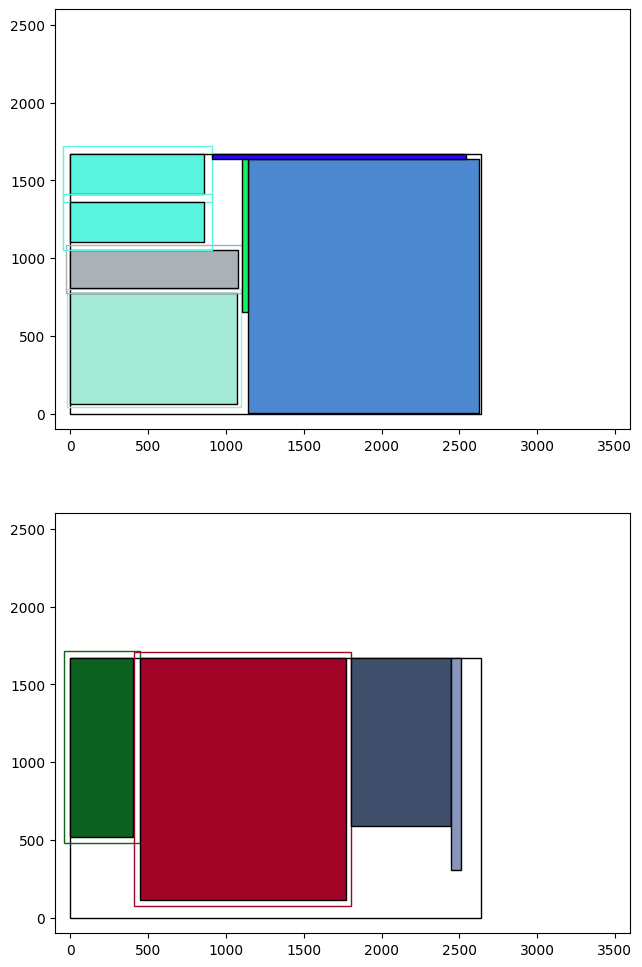
\includegraphics[width=1\columnwidth]{tesi/output} 
    \caption{Esempio nest di una soluzione}
\end{figure}




% \intro{Breve introduzione al capitolo}\\

% \section{Tecnologie e strumenti}
% \label{sec:tecnologie-strumenti}

% Di seguito viene data una panoramica delle tecnologie e strumenti utilizzati.

% \subsection*{Tecnologia 1}
% Descrizione Tecnologia 1.

% \subsection*{Tecnologia 2}
% Descrizione Tecnologia 2

% \section{Ciclo di vita del software}
% \label{sec:ciclo-vita-software}

% \section{Progettazione}
% \label{sec:progettazione}

% \subsubsection{Namespace 1} %**************************
% Descrizione namespace 1.

% \begin{namespacedesc}
%     \classdesc{Classe 1}{Descrizione classe 1}
%     \classdesc{Classe 2}{Descrizione classe 2}
% \end{namespacedesc}


% \section{Design Pattern utilizzati}

% \section{Codifica}

    \chapter{Test computazionali}
\label{cap:verifica-validazione}

\section{Caratteristiche delle istanze}

Le classi di istanze utilizzate per i test computazionali dell'algoritmo sono caratterizzate da una combinazione di parametri che definiscono la complessità e la struttura del problema. Ogni classe rappresenta un insieme di configurazioni che variano in base al numero di oggetti obbligatori (\emph{n\_compulsory}), opzionali (\emph{n\_optional}), formati disponibili (\emph{n\_formats}), margini di sicurezza (\emph{n\_margins}) e vincoli di precedenza (\emph{n\_precs}). Questi parametri sono descritti come segue:

\begin{itemize}
    \item \textbf{Numero di oggetti obbligatori (\emph{n\_compulsory})}: 5, 10, 15 o 20, indicando quanti oggetti devono essere necessariamente posizionati.
    \item \textbf{Numero di oggetti opzionali (\emph{n\_optional})}: 0, 1/3 o 2/3 del numero di oggetti obbligatori della stessa istanza.
    \item \textbf{Numero di formati (\emph{n\_formats})}: tutte le istanze hanno un unico formato disponibile che non è lo stesso per tutte le istanze.
    \item \textbf{Numero di margini di sicurezza (\emph{n\_margins})}: rappresenta il numero di oggetti che richiedono margini di sicurezza, corrisponde a 0, 1/2 o tutti gli oggetti obbligatori della stessa istanza.
    \item \textbf{Numero di vincoli di precedenza (\emph{n\_precs})}: per ogni istanza o tutti gli oggetti obbligatori hanno precedenza o nessuno. 
\end{itemize}

Le classi di istanze sono organizzate per coprire una gamma di complessità crescenti. Le prime configurazioni includono pochi elementi obbligatori, mentre le classi successive incrementano gradualmente il numero di oggetti obbligatori, aumentando il livello di difficoltà del problema. Questa diversificazione permette di valutare l'efficacia dell'algoritmo in scenari con diverse configurazioni geometriche, vincoli di precedenza e complessità computazionale. 

72 classi di istanze da 10 istanze ciascuna.

Totale: 720 istanze.

\section{Configurazione test}

Il test è stato fatto eseguendo l'algoritmo genetico, per tutte le 720 istanze, configurato con la Conf3 (per i motivi citati nella sezione 5.2.1):
\begin{itemize}
    \item\textbf{population\_size}: 50;
	\item\textbf{crossover\_prob}: 0,7 (70\%);
	\item\textbf{mutation\_prob}: 0,3 (30\%);
	\item\textbf{mating\_pool\_size}: 30;
	\item\textbf{elite\_size}: 5.
\end{itemize}
Inoltre, è stato impostando il parametro di \emph{pilot\_method\_prob} a 0,1 (max 10\& dei cromosomi verranno decodificati con il criterio di valutazione \emph{PILOT\_METHOD}) e il criterio di ordinamento della popolazione iniziale \emph{AREA\_DESCENDING} (dall'\emph{item} con area maggiore a quello con area minore).

\section{Risultati}

Il confronto con la soluzione aziendale è fatto prendendo la soluzione migliore ottenuta per ogni istanza dal genetico e la soluzione migliore ottenuta per ogni istanza dalla soluzione aziendale.

Dalle due soluzioni viene confrontata la quantità di scarto totale prodotto:
\begin{itemize}
    \item 56 istanze eseguite con GA hanno ottenuto una soluzione che ha prodotto meno scarto rispetto dalla soluzione aziendale.
    \item 535 istanze hanno ottenuro lo stesso risultato.
    \item 129 istanze hanno ottenuto un risultato peggiore rispetto alla soluzione aziendale.
\end{itemize}

Quindi complessivamente la soluzione aziendale produce un maggior numero di soluzioni migliori per le istanze usate per il confronto.

\subsection{Altri test}

È stato tentato anche un aumento del \emph{pilot\_method\_prob} a 0,5 (50\%) ma ha prodotto risultati peggiori, infatti l'aumento del costo computazionale per l'esecuzione di ogni generazione, rispettando il criterio di arresto a 30 secondi, non ha permesso per alcune istanze di generare abbastanza generazioni per trovare soluzioni migliri che invece, con \emph{pilot\_method\_prob} uguale a 0,1 erano state trovate.

Nella generazione della popolazione iniziale sono stati provati anche altri criteri di ordinamento oltre ad \emph{AREA\_DESCENDING}, come: \emph{LONGER\_SIDE\_DESCENDING} (dal lato lungo maggiore a quello minore), \emph{PERIMETER\_DESCENDING} (dal perimetro maggiore al miniore) e \emph{SIDE\_DIFF\_DESCENDING} (dall'\emph{item} con meno differenza fra altezza e lunghezza a quello con più differenza). Questi criteri di ordinamento hanno ottenuto risultati peggiori (anche utilizzati in combinazione fra di loro e con \emph{AREA\_DESCENDING}) quindi sono stati scartati.
    \chapter{Conclusioni}
\label{cap:conclusioni}

\intro{Nel capitolo finale è presente un resoconto delle attività svolte e degli obiettivi raggiunti. Inoltre è presente una valutazione personale dello stage e delle conoscenze acquisite}

\section{Consuntivo finale}

Nella Tabella 7.1 è presente la tabella di valutazione oraria finale.

\begin{table}[H]
    \centering
    \begin{tabular}{|l|c|c|}
    \hline
    \textbf{Attività} & \textbf{Ore previste} & \textbf{Ore svolte} \\  \hline
    Studio della letteratura & 30 & 40 \\  \hline
    Studio delle tecnologie & 10 & 10 \\  \hline
    Definizione e analisi del problema & 60 & 44 \\  \hline
    Progetto e sviluppo algoritmo genetico & 130 & 120 \\  \hline
    Test e analisi statistica & 44 & 70 \\  \hline
    Stesura documentazione codice & 30 & 20 \\  \hline
    \textbf{Totale} & \textbf{304} & \textbf{304} \\  \hline
    \end{tabular}
    \caption{Consuntivo finale delle attività}
\end{table}

Il livello avnzato dell'argomento trattato nel campo della Ricerca Operativa ha reso necessario l'impiego di più tempo per prendere familiarità con le nozioni di base necessarie, le fasi di sviluppo e analisi degli algoritmi esistenti sono state più agevoli. Infine, la fase di test ha richiesto molto più tempo del necessario a causa dei tempi necesari per la calbrazione dei parametri del GA della configurazione. La stesura della documentazione ha invece richiesto meno tempo del previsto. Complessivamente, i tempi totali sono stati rispettati.

\section{Raggiungimento degli obiettivi}

Nella Tabella 7.2 sono elencati gli obiettivi e il raggiungimento o meno di tale obiettivo.

\begin{table}[H]
    \centering
    \begin{tabular}{|c|c|}
    \hline
    \textbf{Obiettivo} & \textbf{Raggiunto} \\ \hline
    OB1 & Si \\ \hline
    OB2 & Si \\ \hline
    OB3 & Si \\ \hline
    OB4 & Si \\ \hline
    OB5 & Si \\ \hline
    OB6 & Si \\ \hline
    OB6 & Si \\ \hline
    DE1 & Si \\ \hline
    FA1 & No \\ \hline
    \end{tabular}
    \caption{Raggiungimento obiettivi}
\end{table}

Sono stati raggiunti tutti gli obiettivi obbligatori e desiderabili. Il non raggiungimento dell'obbiettivo facoltativo è dovuto a mancanza di ulteriore tempo.

\section{Conoscenze acquisite}

Lavorando in Salvagnini, ho potuto approfondire le dinamiche tipiche di un contesto progettuale e comprendere le sfide legate all'ottimizzazione e alla gestione delle risorse in ambito aziendale. Ho acquisito una chiara consapevolezza di quanto siano cruciali fattori come il tempo, la sincronizzazione e l'efficienza per il successo operativo. In un ambiente competitivo, il miglioramento continuo è una priorità fondamentale, e ciò richiede la capacità di analizzare con attenzione le esigenze e le criticità, adottando un approccio creativo e proattivo per proporre soluzioni innovative e sostenibili.

Dal punto di vista informatico, questa esperienza mi ha permesso di approfondire le mie competenze in Python, sfruttando la sua potenza per sviluppare e ottimizzare algoritmi genetici. Ho potuto applicare in modo concreto le nozioni teoriche apprese durante il mio percorso di studi, specialmente nell'ambito della Ricerca Operativa, traducendole in soluzioni pratiche per problemi reali. L'implementazione dell'algoritmo genetico mi ha permesso di esplorare concetti avanzati di ottimizzazione e di toccare con mano l’efficacia di questi strumenti nel risolvere problemi complessi.

Questa esperienza mi ha dato anche l'opportunità di migliorare le mie capacità di programmazione e di approfondire l'importanza della creatività e dell'innovazione nel mondo dello sviluppo software, fornendomi una base solida per affrontare progetti futuri con un approccio analitico e orientato al risultato.

\section{Valutazione personale}

La complessità del progetto e la necessità di affacciarmi a un mondo, quello degli algoritmi evolutivi, che non conoscevo mi ha inizialmente richiesto del tempo per abituarmi. Tuttavia, questa sfida si è rivelata un'opportunità unica per approfondire la mia conoscenza di Python e delle tecniche di ottimizzazione, scoprendo tecnologie e approcci che non conoscevo. Il bisogno di approfondire la conoscenza teorica e di scegliere i corretti elementi per lo sviluppo dell'algoritmo genetico ha sicuramente potenziato le mie capacità di problem solving e il mio spirito critico.

L'esperienza maturata in azienda ha un riscontro assolutamente positivo, da subito mi sono trovato in un ambiente di lavoro sereno e stimolante. La collaborazione con il tutor aziendale è stata importantissima, mi ha permesso di affacciarmi a un mondo lavorativo professionale e una visone del progetto molto più analitica.

Riguardo al progetto, ritengo che l'algoritmo genetico abbia un potenziale notevole per risolvere problemi complessi, ma che necessiti di un'attenta analisi per essere applicato al meglio in contesti reali. È un approccio che, pur essendo molto potente, richiede una comprensione profonda dei problemi da risolvere e delle soluzioni da implementare. Per ottenere i migliori risultati, sarebbe utile il coinvolgimento di un team con competenze diversificate e di esperti che possano guidare la scelta delle strategie più efficaci in base agli obiettivi specifici.

Nel complesso, questa esperienza ha avuto un esito estremamente positivo. Mi ha permesso di raggiungere risultati concreti, di ampliare le mie competenze in ambito di ottimizzazione e programmazione, e di comprendere meglio le necessità di un progetto complesso.

    \appendix
    \chapter{Appendice A}

\epigraph{Citazione}{Autore della citazione}


    \backmatter
    \printglossary[type=\acronymtype, title=Acronimi e abbreviazioni, toctitle=Acronimi e abbreviazioni]
    \printglossary[type=main, title=Glossario, toctitle=Glossario]

    \cleardoublepage
\chapter{Bibliografia}

\nocite{*}

% Print book bibliography
\printbibliography[heading=subbibliography,title={Riferimenti bibliografici},type=book]

% Print site bibliography
\printbibliography[heading=subbibliography,title={Siti web consultati},type=online]

\end{document}
